\chapter{Aplicaciones del cálculo científico al álgebra lineal}
\section{Matrices y vectores}
En esta sección vamos a repasar algunos conceptos fundamentales de  álgebra lineal y cómo pueden manejarse empleando Matlab. No daremos definiciones precisas ni tampoco demostraciones, ya que tanto unas como otras se verán en detalle en la asignatura de álgebra. 
\paragraph{matrices.} Desde un punto de vista funcional definiremos una matriz como una tabla bidimensional de números ordenados en filas y columnas,
\begin{equation*}
A=
\begin{pmatrix}
1& \sqrt(2)& 3.5& 0\\
-2& \pi& -4.6& 4\\
7& -19& 2.8& 0.6
\end{pmatrix}
\end{equation*}

Cada línea horizontal de números constituye una \emph{fila} de la matriz y cada línea horizontal una \emph{columna} de la misma.

A una matriz con $m$ filas y $n$ columnas se la denomina matriz de orden $m\times n$. $m$ y $n$ son la dimensiones de la matriz y se dan siempre en el mismo orden: primero el número de filas y después el de columnas. Así, la matriz $A$ del ejemplo anterior es una matriz $3\times 4$. El orden de una matriz expresa el tamaño de la matriz.

Dos matrices son iguales si tienen el mismo orden, y los elementos que ocupan en ambas matrices los mismo lugares son iguales.

Una matriz es cuadrada, si tiene el mismo número de filas que de columnas. Es decir es de orden $n\times n$.

Mientras no se diga expresamente lo contrario, emplearemos letras mayúsculas $A, B, \cdots$ para representar matrices. La expresión $A_{m\times n}$ indica que la matriz $A$ tiene dimensiones $m \times n$. Para denotar los elementos de una matriz, emplearemos la misma letra en minúsculas empleada para nombrar la matriz, indicando mediante subíndices, y siempre por este orden, la fila y la columna a la que pertenece el elemento. Así por ejemplo $a_{ij}$ representa al elemento de la matriz $A$, que ocupa la fila $i$ y la columna $j$.

\begin{equation*}
A=
\begin{pmatrix}
1& \sqrt(2)& 3.5& 0\\
-2& \pi& -4.6& 4\\
7& -19& 2.8& 0.6
\end{pmatrix}
\rightarrow a_{23}=-4.6
\end{equation*}

\paragraph{vectores}
A una matriz compuesta por una sola fila, la denominaremos vector fila. A una matriz compuesta por una sola columna la denominaremos vector columna. Siempre que hablemos de un vector, sin especificar más, entenderemos que se trata de un vector columna.\footnote{Esta identificación de los vectores como vectores columna no es general. La introducimos porque simplifica las explicaciones posteriores.} Para representar vectores, emplearemos letras minúsculas. Para representar sus elementos añadiremos a la letra que representa al vector un subíndice indicando la fila a la que pertenece el elemento.

\begin{equation*}
a=
\begin{pmatrix}
a_1\\
a_2\\
\vdots \\
a_i\\
\vdots \\
a_n
\end{pmatrix}
\end{equation*}

Podemos asociar los puntos del plano con los vectores de dimensión dos. Para ello, usamos una representación cartesiana, en la que los elementos del vector son los valores de las coordenadas $(x,y)$ del punto del plano que representan. Cada vector se representa gráficamente mediante una flecha que parte del origen de coordenadas y termina en el punto $(x,y)$ representado por el vector. La figura \ref{fig:vectores} representa los vectores,
\begin{equation*}
a=
\begin{pmatrix}
1\\
2
\end{pmatrix},
b=
\begin{pmatrix}
2\\
-3
\end{pmatrix},
c=
\begin{pmatrix}
0\\
-2
\end{pmatrix}
\end{equation*}


\begin{figure}[h]
\centering
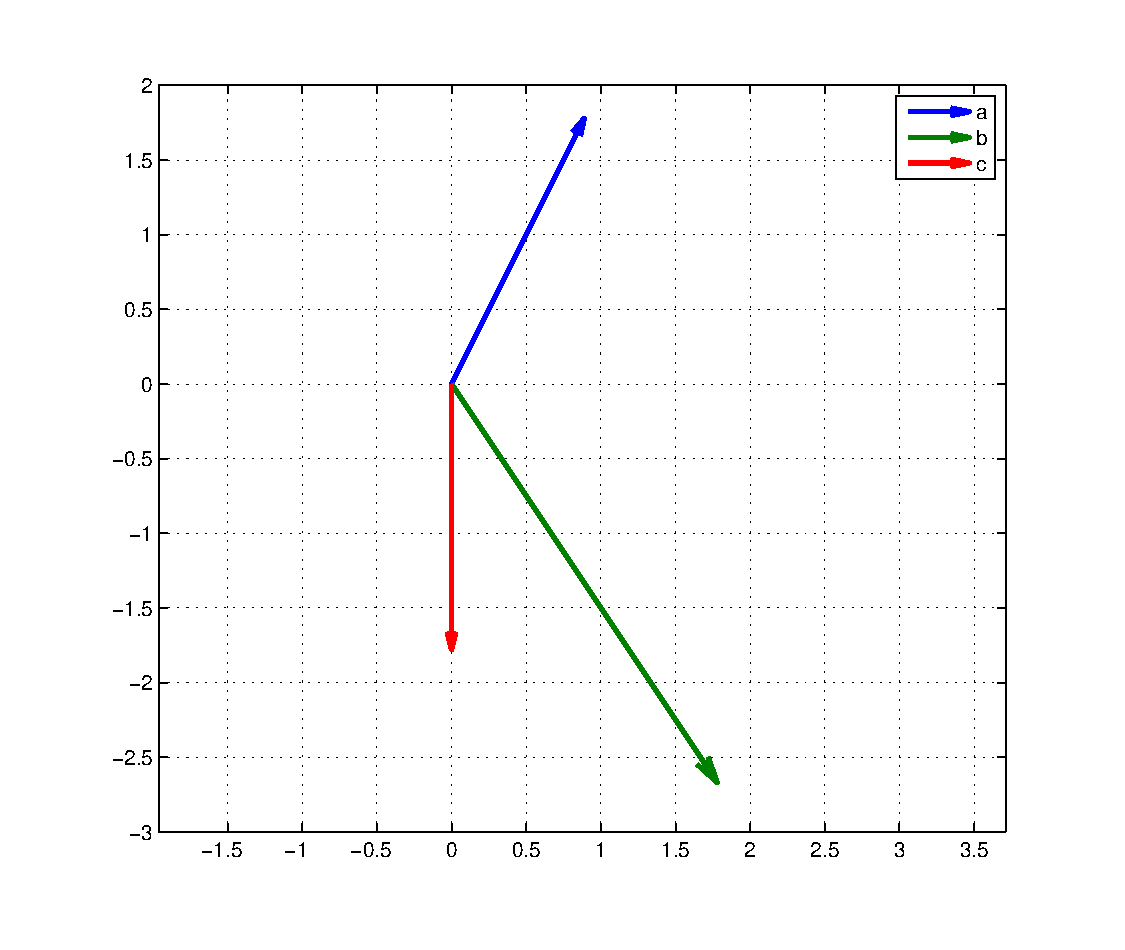
\includegraphics[width=7cm]{vectores.eps}
\caption{Representación gráfica de vectores en el plano}
\label{fig:vectores}
\end{figure}

De modo análogo, podemos asociar vectores de dimensión tres con puntos en el espacio tridimensional. En este caso, los valores de los elementos del vector corresponden con la coordenadas $(x,y,z)$ de los puntos en el espacio. La figura \ref{fig:vectores3} muestra la representación gráfica en espacio tridimensional de los vectores, 
\begin{equation*}
a=
\begin{pmatrix}
1\\
2\\
1
\end{pmatrix},
b=
\begin{pmatrix}
2\\
-3\\
-1
\end{pmatrix},
c=
\begin{pmatrix}
0\\
-2\\
1
\end{pmatrix}
\end{equation*}

\begin{figure}[h]
\centering
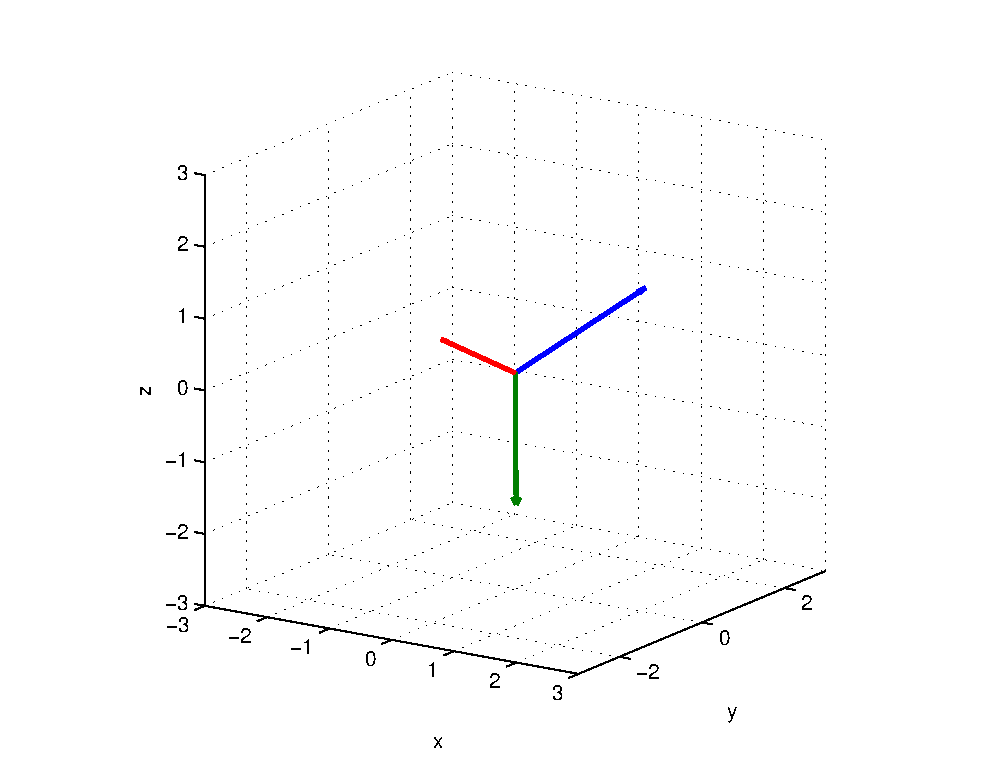
\includegraphics[width=9cm]{vectores3.eps}
\caption{Representación gráfica de vectores en el espacio}
\label{fig:vectores3}
\end{figure}

Evidentemente para vectores de mayor dimensión, no es posible obtener una representación gráfica. Si embargo muchas de las propiedades geométricas, observables en los vectores bi y tridimensionales, pueden extrapolarse a vectores de cualquier dimensión.



\section{Operaciones matriciales}\label{opmatr}

A continuación definiremos las operaciones matemáticas más comunes, definidas sobre matrices. 

\paragraph{suma.} La suma de dos matrices, se define como la matriz resultante de sumar los elementos que ocupan en ambas la misma posición. Solo está definida para matrices del mismo orden,

\begin{gather*}
C=A+B\\
c_{ij}=a_{ij}+b_{ij}\\
\\
\begin{pmatrix}
1& 2& 3\\
4& 5& 6\\
7& 8& 9\\
\end{pmatrix} =
\begin{pmatrix}
1& 3& 5\\
3& 5& 7\\
5& 7& 9\\
\end{pmatrix} +
\begin{pmatrix}
0& -1& -2\\
1& 0& -1\\
2& 1& 0\\
\end{pmatrix}
\end{gather*}

La suma de matrices cumple las siguientes propiedades,
\begin{enumerate}
\item Asociativa: $(A+B)+C=A+(B+C)$
\item Conmutativa: $A+B=B+A$
\item Elemento neutro: $O_{n\times m}+A_{n\times m}=A_{m\times m}$ El elemento neutro $O_{n\times m}$ de la suma de matrices de orden $n\times m$ es la matriz nula de dicho orden, ---compuesta exclusivamente por ceros--- . 

En Matlab, podemos crear una matriz de cualquier orden, compuesta exclusivamente por ceros mediante el comando \texttt{zeros(m,n)}, donde $m$ es el número de filas y $n$ el de columnas de la matriz de ceros resultante,

\begin{verbatim}
>> O=zeros(2,3)
O =
     0     0     0
     0     0     0
>> A=[1 2 3; 4 3 6]
A =
     1     2     3
     4     3     6
>> B=A+O
B =
     1     2     3
     4     3     6
>> 
\end{verbatim}
\item Elemento opuesto: La opuesta a una matriz se obtiene cambiando de signo todos sus elementos, $A_{op}=-A$

\begin{verbatim}
>> A
A =
     1     2     3
     4     3     6
>> Aop=-A
Aop =
    -1    -2    -3
    -4    -3    -6
>> S=A+Aop
S =
     0     0     0
     0     0     0
\end{verbatim}
\end{enumerate}
En Matlab el signo $+$ representa por defecto la suma de matrices, por lo que la suma de dos matrices puede obtenerse directamente como, 

\begin{verbatim}
>> A=[1 2 3; 4 3 6]
A =
     1     2     3
     4     3     6
>> B=[1 2 3; 4 -3 2]
B =
     1     2     3
     4    -3     2
>> S=A+B
S =
     2     4     6
     8     0     8
\end{verbatim}



\paragraph{Transposición}
Dada una matriz $A$, su transpuesta $A^T$ se define como la matriz que se obtiene intercambiando sus filas con sus columnas,

\begin{gather*}
A \rightarrow  A^T\\
a_{ij} \rightarrow  a_{ji}\\
A=
\begin{pmatrix}
1& -3& 2 \\
2& 7& -1
\end{pmatrix}  \rightarrow 
A^T=
\begin{pmatrix}
1& 2 \\
-3& 7\\
2 & -1
\end{pmatrix}
\end{gather*}

En Matlab, la operación de transposición se indica mediante un apóstrofo ('),

\begin{verbatim}
>> A=[1 2 3; 4 3 6]
A =
     1     2     3
     4     3     6
>> B=A'
B =
     1     4
     2     3
     3     6
\end{verbatim}

Para vectores, la transposición convierte un vector fila en un vector columna y viceversa. 
\begin{gather*}
a \rightarrow a^T\\
a=
\begin{pmatrix}
1 \\
-3\\
2 
\end{pmatrix}
 \rightarrow 
a^T=
\begin{pmatrix}
1& -3 & 2 
\end{pmatrix} 
\end{gather*}

Una matriz cuadrada se dice que es simétrica si coincide con su transpuesta,

\begin{gather*}
A=A^T\\
a_{ij}=a{ji}\\
A=A^T=
\begin{pmatrix}
\ 1&\ 3&-3\\
\ 3&\ 0&-2\\
-3&-2&\ 4
\end{pmatrix}
\end{gather*}

Una matriz cuadrada es antisimétrica cuando cumple que $A=-A^T$. Cualquier matriz cuadrada se puede descomponer en la suma de una matriz simétrica más otra antisimétrica.

La parte simétrica puede definirse como,
\begin{equation*}
A_S=\frac{1}{2} \left( A+A^T \right)
\end{equation*}

y la parte antisimétrica como,

\begin{equation*}
A_A=\frac{1}{2}\left( A-A^T \right)
\end{equation*}

Así, por ejemplo,

\begin{equation*}
 A=A_S+A_A \rightarrow
\begin{pmatrix}
1& 2& 3\\
4& 5& 6\\
7& 8& 9\\
\end{pmatrix} =
\begin{pmatrix}
1& 3& 5\\
3& 5& 7\\
5& 7& 9\\
\end{pmatrix} +
\begin{pmatrix}
0& -1& -2\\
1& 0& -1\\
2& 1& 0\\
\end{pmatrix}
\end{equation*}

Por último, la transpuesta de la suma de matrices cumple,
\begin{equation*}
(A+B)^T=A^T+B^T
\end{equation*}


\paragraph{Producto de una matriz por un escalar.} El producto de una matriz $A$ por un número $b$ es una matriz del mismo orden que $A$, cuyos elementos se obtienen multiplicando los elementos de $A$ por el número $b$,

\begin{gather*}
C=b\cdot A \rightarrow c_{ij}=b\cdot a_{ij}\\
3\cdot
\begin{pmatrix}
1& -2& 0\\
2& 3& -1&
\end{pmatrix}=
\begin{pmatrix}
3& -6& 0\\
6& 9& -3&
\end{pmatrix} 
\end{gather*}
En Matlab, el símbolo \texttt{*} se emplea para representar el producto entre escalares (números), entre escalares y matrices y el producto entre matrices, como veremos en los siguientes párrafos.

\paragraph{Producto escalar de dos vectores.} Dados vectores de la misma dimensión $m$ se define su producto escalar como, 

\begin{gather*}
a\cdot b=\sum_{i=1}^na_ib_i\\
\begin{pmatrix}
1\\
3\\
4
\end{pmatrix}\cdot
\begin{pmatrix}
1\\
-2\\
0
\end{pmatrix}
=1\cdot 1+3 \cdot (-2)+ 4 \cdot 0= -5
\end{gather*}

El resultado de producto escalar de dos vectores, es siempre un número; se multiplican los entre sí los elementos de los vectores que ocupan idénticas posiciones y se suman los productos resultantes. 


\paragraph{Producto matricial}
El producto de una matriz de orden $n\times m$ por una matriz $m\times l$, es una nueva matriz de orden $n\times l$, cuyos elementos se obtiene de acuerdo con la siguiente expresión,

\begin{equation*}
P=A\cdot B \rightarrow a_{ij}=\sum_{t=1}^m a_{it}b_{tj}
\end{equation*}

Por tanto, el elemento de la matriz producto que ocupa la fila i y la columna j, se obtiene multiplicando por orden los elementos de la fila i de la matriz A con los elementos correspondientes de la columna j de la matriz B, y sumando los productos resultantes.

Para que dos matrices puedan multiplicarse es imprescindible que el número de columnas de la primera matriz coincida con el número de filas de la segunda.

Podemos entender la mecánica del producto de matrices de una manera más fácil si consideramos  la primera matriz como un grupo de vectores fila,
\begin{equation*}
\begin{aligned}
A_1=\begin{pmatrix}
a_{11}& a_{12}& \cdots a_{1n}
\end{pmatrix}\\
A_2=\begin{pmatrix}
a_{21}& a_{22}& \cdots a_{2n}
\end{pmatrix}\\
\vdots \  \ \   \  \  \  \ \ \ \ \\
A_m=\begin{pmatrix}
a_{m1}& a_{m2}& \cdots a_{mn}
\end{pmatrix}
\end{aligned} \ \rightarrow \ 
A=\begin{pmatrix}
a_{11}& a_{12}& \cdots a_{1n}\\
a_{21}& a_{22}& \cdots a_{2n}\\
\vdots& \vdots& \cdots& \vdots \\
a_{m1}& a_{m2}& \cdots a_{mn}
\end{pmatrix}
\end{equation*}
y la segunda matriz como un grupo de vectores columna,

\begin{equation*}
\begin{aligned}
B_1=\begin{pmatrix}
b_{11}\\ b_{21}\\ \vdots \\ b_{n1}
\end{pmatrix}&
B_2=\begin{pmatrix}
b_{12}\\ b_{22}\\ \vdots\\ b_{n2}
\end{pmatrix} &
\cdots  \  \  &
B_3=\begin{pmatrix}
b_{1m}\\ b_{2m}\\ \vdots  b_{nm}
\end{pmatrix}
\end{aligned} \ \rightarrow \ 
B=\begin{pmatrix}
b_{11}& b_{12}& \cdots b_{1n}\\
b_{21}& b_{22}& \cdots b_{2n}\\
\vdots& \vdots& \cdots& \vdots \\
b_{m1}& b_{m2}& \cdots b_{mn}
\end{pmatrix}
\end{equation*}

Podemos ahora considerar  cada elemento $p_{ij}$ de la matriz producto $P=A\cdot B$ como el producto escalar del vector fila $A_i$ for el vector columna $B_j$, $p_{ij}=A_i\cdot B_j$. 
Es ahora relativamente fácil, deducir algunas de las propiedad del producto matricial,

\begin{enumerate}
\item Para que dos matrices puedan multiplicarse, es preciso que el número de columnas de la primera coincida con el numero de filas de la segunda. Además la matriz producto tiene tantas filas como la primera matriz y tantas columnas como la segunda.

\item El producto matricial no es conmutativo. En general $A\cdot B \neq B \cdot A$

\item $(A\cdot B)^T=B^T\cdot A^T$
\end{enumerate}

\paragraph{Matriz identidad} La matriz identidad de orden $n\times n$ se 
define como:
\begin{equation*}
I_n= \left\{ 
\begin{aligned}
i_{ll}&=1\\
i_{kj}&=0, \ k\neq j
\end{aligned}
\right.
\end{equation*}

Es decir, una matriz en la que todos los elementos que no pertenecen a la diagonal principal son $0$ y los elementos de la diagonal principal son $1$. Por ejemplo,

\begin{equation*}
I_3=\begin{pmatrix}
1& 0& 0\\
0& 1& 0\\
0& 0& 1
\end{pmatrix}
\end{equation*}
La matriz identidad $I_n$ es el elemento neutro del producto de matrices cuadradas de orden $n\times n$,
\begin{equation*}
A_{n\times n}\cdot I_n=I_n\cdot A_{n\times n}
\end{equation*}

Además,
\begin{gather*}
A_{n\times m}\cdot I_m=A_{n \times m}\\
I_n\cdot A_{n\times m}=A_{n\times m}
\end{gather*}

En Matlab se emplea el comando \texttt{eye(n)} para construir la matriz identidad de orden $n\times n$,

\begin{verbatim}
>> I4=eye(4)
I4 =
     1     0     0     0
     0     1     0     0
     0     0     1     0
     0     0     0     1
\end{verbatim}

Una matriz cuadrada se dice que es ortogonal si cumple,
\begin{equation*}
A^T\cdot A=I
\end{equation*}

\paragraph{Producto escalar de dos vectores y producto matricial} Por conveniencia,  representaremos el producto escalar de dos vectores como un producto matricial,

\begin{gather*}
a\cdot b= a^Tb=b^Ta=b\cdot a\\
\begin{pmatrix}
1& 3& 4
\end{pmatrix}
\begin{pmatrix}
1\\
-2\\
0
\end{pmatrix}
=
\begin{pmatrix}
1& -1& 0
\end{pmatrix}
\begin{pmatrix}
1\\
3\\
4
\end{pmatrix}
=1\cdot 1+3 \cdot (-2)+ 4 \cdot 0= -5
\end{gather*}

Es decir, transponemos el primer vector del producto, convirtiéndolo en un vector fila.

\paragraph{Norma de un vector.} La longitud euclídea, módulo,  norma 2 o simplemente norma  de un vector se define como,

\begin{equation*}
\Vert x \Vert_2 =\Vert x \Vert =\sqrt{x\cdot x}=\sqrt{x^Tx}=\sqrt{x_1^2+x_2^2+\cdots x_n^2}=\left( \sum_{i=1}^nx_i^2 \right)^\frac{1}{2}
\end{equation*}

Constituye la manera usual de medir la longitud de un vector. Tiene una interpretación geométrica inmediata a través del teorema de Pitágoras: nos da la longitud del segmento que representa al vector. La figura \ref{fig:pitag} muestra dicha interpretación, para un vector bidimensional.  

\begin{figure}[h]
\centering
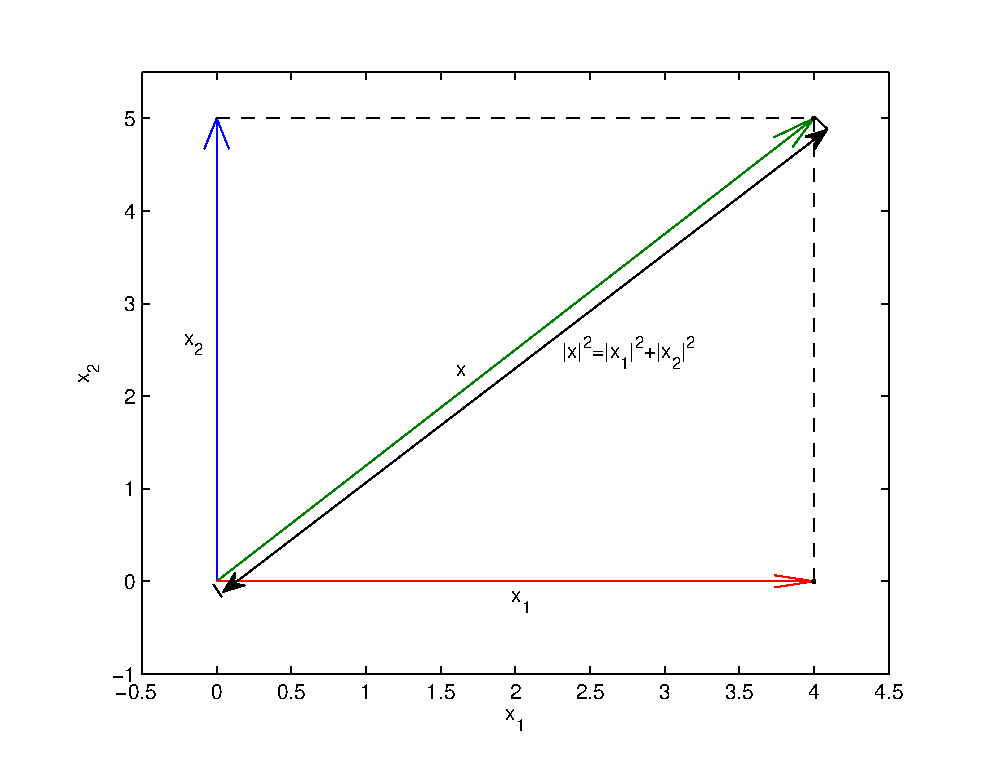
\includegraphics[width=12cm]{pitag.eps}
\caption{interpretación geométrica de la norma de un vector}
\label{fig:pitag}
\end{figure}

A partir de la norma de un vector es posible obtener una expresión alternativa para el producto escalar de dos vectores,
\begin{equation*}
a\cdot b=\Vert a \Vert \Vert b \Vert \cos \theta
\end{equation*}
Donde $\theta$ representa el ángulo formado por los dos vectores.

Aunque se trate de la manera más común de definir la norma de un vector, la norma 2 no es la única definición posible,

\begin{itemize}
\item Norma 1: Se define como la suma de los valores absolutos de los elementos de un vector,
\begin{equation*}
\Vert x \Vert_1 =\vert x_1\vert +\vert x_2 \vert\cdots \vert x_n\vert
\end{equation*}
\item Norma p, Es una generalización de la norma 2,
\begin{equation*}
\Vert x \Vert_p =\sqrt[p]{\vert x_1^p\vert+\vert x_2^p\vert+\cdots \vert x_n^p\vert}=\left( \sum_{i=1}^n\vert x_i^p \vert \right)^\frac{1}{p}
\end{equation*}
\item norma $\infty$, se define como el mayor elemento del vector valor absoluto,

\begin{equation*}
\Vert x \Vert_\infty =max \left\lbrace \vert x_i\vert\right \rbrace 
\end{equation*}

\item Norma $-\infty$, el menor elemento del vector en valor absoluto,
 
\begin{equation*}
\Vert x \Vert_{-\infty} =min \left\lbrace \vert x_i\vert\right \rbrace 
\end{equation*}
\end{itemize}

En Matlab la norma de un vector puede obtenerse mediante el comando \texttt{norm(v,p)} La primera variable de entrada debe ser un vector y la segunda el tipo de norma que se desea calcular. Si se omite la segunda variable de entrada, el comando devuelve la norma 2. A continuación se incluyen varios ejemplo de utilización,
\begin{verbatim}
>> x=[1;2;-3;0;-1]
x =
     1
     2
    -3
     0
    -1
>> norma_2=norm(x,2)
norma_2 =
     3.872983346207417e+00
>> norma=norm(x)
norma =
     3.872983346207417e+00
>> norma_1=norm(x,1)
norma_1 =
     7
>> norma_4=norm(x,4)
norma_4 =
     3.154342145529904e+00
>> norma_inf=norm(x,inf)
norma_inf =
     3
>> norma_minf=norm(x,-inf)
norma_minf =
     0
\end{verbatim} 

En general, una norma se define como una función de $\mathbb{R}^n \rightarrow \mathbb{R}$, que cumple,
\begin{align*}
&\Vert x\Vert \geq 0,\  \Vert x\Vert =0 \Rightarrow x=0\\
&\Vert x+y\Vert \leq \Vert x\Vert +\Vert y\Vert \\
&\Vert \alpha x\Vert = \vert \alpha \vert \Vert x\Vert ,\ \alpha \in \mathbb{R} 
\end{align*}

Llamaremos vectores unitarios $u$, a aquellos para los que se cumple que $\Vert u \Vert=1$.

Dos vectores $a$ y $b$ son ortogonales si cumplen que su producto escalar es nulo, $a^Tb=0 \Rightarrow  a\bot b$. Si además ambos vectores tienen módulo unidad, se dice entonces que los vectores son ortonormales.  Desde el punto de vista de su representación geométrica, dos vectores ortogonales, forman entre sí un ángulo recto.

\paragraph{Traza de una matriz.} La traza de una matriz cuadrada , se define como la suma de los elementos que ocupan su diagonal principal, 
\begin{gather*}
Tr(A)=\sum_{i=1}^na_{ii}\\
Tr\left(
\begin{pmatrix}
1& 4 & 4\\
2& -2 & 2\\
0& 3 & 6
\end{pmatrix}\right)=1-2+6=5
\end{gather*}

La traza de la suma de dos matrices cuadradas $A$ y $B$ del mismo orden, coincide con la suma de las trazas de $A$ y $B$,
\begin{equation*}
tr(A+B)=tr(A)+tr(B)
\end{equation*}

Dada una  matriz $A$ de dimensión $m\times n$  y una matriz $B$ de dimensión $n \times m$, se  cumple que,
\begin{equation*}
tr(AB)=tr(BA)
\end{equation*}

En Matlab, puede obtenerse directamente el valor de la traza de una matriz, mediante el comando \texttt{trace},
\begin{verbatim}
>> A=[1 3 4
3  5 2
2 -1 -2]
A =
     1     3     4
     3     5     2
     2    -1    -2
>> t=trace(A)
t =
     4
\end{verbatim}

\paragraph{Determinante de una matriz.} El determinante de una matriz $A$, se representa habitualmente como $\vert A \vert$ o, en ocasiones como $det(A)$. Para poder definir el determinante de una matriz, necesitamos antes introducir una serie de conceptos previos. En primer lugar, si consideramos un escalar como una matriz de un solo elemento, el determinante  sería precisamente el valor de ese único elemento,
\begin{equation*}
A=\begin{pmatrix}
a_{11}
\end{pmatrix} \rightarrow \vert A \vert =a_{11}
\end{equation*}

Se denomina menor complementario o simplemente menor, $M_{ij}$ del elemento $a_{ij}$ de una matriz $A$, a la matriz que resulta de eliminar de la matriz $A$ la fila $i$ y la columna $j$ a las que pertenece el elemento $a_{ij}$. Por ejemplo,
\begin{align*}
A=\begin{pmatrix}
1& 0& -2\\
3& -2& 3\\
0& 6& 5
\end{pmatrix},& \ 
M_{23}=
\begin{pmatrix}
1& 0\\
0& 6
\end{pmatrix}\\
M_{32}=
\begin{pmatrix}
1& -2\\
3& 3
\end{pmatrix},& \ 
M_{33}=
\begin{pmatrix}
1& 0\\
3& -2
\end{pmatrix}\cdots
\end{align*}

 El  cofactor $C_{ij}$ de un elemento $a_{ij}$ de la matriz $A$, se define a partir del determinante del menor complementario del elemento $a_{ij}$ como,

\begin{equation*}
C_{ij}=(-1)^{i+j}\vert M_{ij} \vert
\end{equation*}

Podemos ahora definir el determinante de una matriz $A$ cuadrada de orden $n$, empleando la fórmula de Laplace, 

\begin{equation*}
\vert A \vert = \sum_{j=1}^n a_{ij}C_{ij}
\end{equation*}

o alternativamente,


\begin{equation*}
\vert A \vert = \sum_{i=1}^n a_{ij}C_{ij}
\end{equation*}

En el primer caso, se dice que se ha desarrollado el determinante a lo largo de la fila $i$. En el segundo caso, se dice que se ha desarrollo el determinante a lo largo de la columna $j$.

 La fórmula de Laplace, obtiene el determinante de una matriz de orden $n\times n$ a partir del cálculo de los determinantes de los menores complementarios de los elementos de una fila; $n$ matrices de orden $(n-1)\times (n-1)$. A su vez, podríamos calcular el determinante de cada menor complementario, aplicando la formula de Laplace y así sucesivamente hasta llegar a matrices de orden $2\times 2$. Para una matriz $2\times 2$, si desarrollamos por la primera fila obtenemos su determinante como,

\begin{align*}
A&=\begin{pmatrix}
a_{11}& a_{12}\\
a_{21}& a_{22}
\end{pmatrix}\\
\vert A \vert & =\sum_{j=1}^2a_{1j}C_{1j} =a_{11}C_{11}+a_{12}C_{12}\\
 &=a_{11}(-1)^{1+1}\vert M_{11}\vert +a_{12}(-1)^{1+2}\vert M_{12}\vert \\
 &=-a_{11}a_{22}+a_{12}a_{21}\\
\end{align*}

y si desarrollamos por la segunda columna,

\begin{align*}
A&=\begin{pmatrix}
a_{11}& a_{12}\\
a_{21}& a_{22}
\end{pmatrix}\\
\vert A \vert & =\sum_{j=1}^2a_{i2}C_{i2} =a_{12}C_{12}+a_{22}C_{22}\\
 &=a_{12}(-1)^{1+2}\vert M_{12}\vert +a_{22}(-1)^{2+2}\vert M_{22}\vert \\
 &=-a_{12}a_{21}+a_{22}a_{12}\\
\end{align*}


Para una matriz de dimensión arbitraria $n\times n$, el determinante se obtiene aplicando recursivamente la fórmula de Laplace,

\begin{align*}
&\vert A  \vert = \sum_{j=1}^na_{ij}C_{ij} =\sum_{j=1}^na_{ij}(-1)^{i+j} \left \vert M_{ij}^{(n-1)\times(n-1)} \right \vert \\
&\left \vert M_{ij}^{(n-1)\times(n-1)} \right \vert = \sum_{k=1}^{n-1}m_{lk}C_{lk} =\sum_{k=1}^{n-1}m_{lk}(-1)^{l+k} \left \vert M_{lk}^{(n-2)\times (n-2)} \right \vert\\
&\vdots \\
&\left \vert M_{st}^{1\times 1}\right \vert=(-1)^{s+t}m_{st} 
\end{align*}

Asi, por ejemplo, podemos calcular el determinante de la matriz,
\begin{equation*}
A=\begin{pmatrix}
1& 0& -2\\
3& -2& 3\\
0& 6& 5
\end{pmatrix}
\end{equation*}
desarrollándolo por los elementos de la primera columna, como,
\begin{align*}
\left\vert A \right\vert =& 1\cdot (-1)^2\cdot 
\left\vert \begin{matrix}
-2& 3\\ 
6& 5
\end{matrix} \right\vert + 3\cdot (-1)^3\cdot
\left\vert \begin{matrix}
0& -2\\ 
6& 5
\end{matrix} \right\vert+ 0\cdot (-1)^4 \cdot 
\left\vert \begin{matrix}
0& -2\\ 
-2& -3
\end{matrix} \right\vert \\
=& 1\cdot (-1)^2\cdot \left[ (-2)\cdot 5 - 6\cdot 3 \right] +3\cdot (-1)^3\cdot  \left[ 0\cdot 5 - 6\cdot (-2)\right] + 0\cdot (-1)^4 \cdot \left[ 0\cdot 3 - (-2)\cdot (-2)\right]= -64
\end{align*}

Podemos programar en Matlab una función recurrente que calcule el determinante de una matriz de rango $n\times n$. (El método no es especialmente eficiente pero ilustra el uso de funciones recursivas.

\begin{verbatim}
function d=determinante(M)
%este programa, calcula el determinante de una matriz empleando la formula
%de Laplace. La función es recursiva, (se llama a si misma sucesivamente
%para calcular los cofactores necesarios). Desarrolla siempre por los
%elementos de la primera columna. (Es un prodigio de ineficiencia numerica,
%pero permite manejar bucles y funciones recursivas, asi que supongo que
%puede ser útil para los que empiezan a programar).
%un posible ejercicio para ver lo malo que es el método, consiste ir
%aumentando la dimension de la matriz y comparar lo que lo tarde en
%calcular el determinante con lo que tarda la función de Matlab det...

%primero comprobamos que la matriz suministrada es cuadrada:
d=0;
[a,b]=size(M);
if a~=b
    disp('la matriz no es cuadrada, Campeón')
    d=[];
else
    for i=1:a
        if a==1
            d=M;
        else
            %Eliminamos la fila y columna que toque
            N=M([1:i-1 i+1:a],2:b);
            %Añadimos el calculo correspondiente al cofactor
            d=(-1)^(i+1)*M(i,1)*determinante(N)+d;
            %pause
        end
    end
end

\end{verbatim}

En Matlab, el determinante de una matriz se calcula directamente empleando la función \texttt{det}. Así, para calcular el determinante de la matriz $A$ del ejemplo anterior,
\begin{verbatim}
>> A=[1 0 -2; 3 -2 3; 0 6 5]
A =

     1     0    -2
     3    -2     3
     0     6     5
>> da=det(A)
da =
   -64
\end{verbatim}

Entre las propiedades de los determinantes, destacaremos las siguientes,
\begin{enumerate}
\item El determinante del producto de un escalar $a$ por una matriz $A$ de dimensión $n\times n$ cumple,
\begin{equation*}
\left\vert a\cdot A \right\vert =a^n\cdot \vert A \vert
\end{equation*}
\item El determinante de una matriz es igual al de su traspuesta,
\begin{equation*}
\vert A \vert =\left\vert A^T \right\vert
\end{equation*}

\item El determinante del producto de dos matrices es igual al producto de los determinantes,
\begin{equation*}
\left\vert A_{n\times n} \cdot  B_{n\times n} \right\vert = \left\vert A_{n\times n} \right\vert \cdot \left\vert B_{n\times n} \right\vert 
\end{equation*}
\end{enumerate}

Una matriz es singular si su determinante es cero.

El rango de una matriz se define como el tamaño de la submatriz más grande dentro de $A$, cuyo determinante es distinto de cero. Así por ejemplo la matriz,
\begin{equation*}
A=\begin{pmatrix}
1& 2& 3\\
4& 5& 6\\
7& 8& 9
\end{pmatrix} \rightarrow \vert A \vert =0
\end{equation*}
Es una matriz singular y su rango es dos,
\begin{equation*}
\begin{matrix}
1& 2\\
4& 5
\end{matrix}=-3 \neq 0 \Rightarrow r(A)=2
\end{equation*}

Para una matriz no singular, su rango coincide con su orden.

En Matlab se puede estimar el rango de una  matriz mediante el comando \texttt{rank},
\begin{verbatim}
>> A=[1 2 3
4 5 6
7 8 9]
A =

     1     2     3
     4     5     6
     7     8     9
>> r=rank(A)
r =
     2
\end{verbatim}

\paragraph{Inversión.} Dada una matriz cuadrada no singular $A$ existe una única matriz $A^{-1}$ que cumple,
\begin{equation*}
A_{n\times n}\cdot A_{n\times n}^{-1}=I_{n\times n}
\end{equation*}

La matriz $A^{-1}$ recibe el nombre de matriz inversa de $A$, y puede calcularse a partir de $A$ como,
\begin{equation*}
A^{-1}=\frac{1}{\vert A \vert}[adj(A)]^T
\end{equation*}

Donde $adj(A)$ es la matriz adjunta de $A$, que se obtiene sustituyendo cada elemento $a_{ij}$ de $A$, por su cofactor $C_{ij}$. A continuación incluimos el código en Matlab de una función \texttt{inversa} que calcula la inversa de una matriz. La función \texttt{inversa} llama a su vez a la función \texttt{determinante} descrita más arriba. Lo ideal es crear un fichero \texttt{inversa.m} que incluya las dos funciones una detrás de la otra tal y como aparecen escritas a continuación. De este modo, si llamamos desde el \emph{workspace} de Matlab a la función \texttt{inversa}, esta encuentra siempre el código de \texttt{deteminante} ya que está contenido en el mimo fichero.

\begin{verbatim}
function B=inversa(A)
%este programa calcula la inversa de una matriz a partir de definición
%típica: A^(-1)=[adj(A)]'/det(A)
%Se ha includo al final del programa una funcion (determinante) para 
%calcular determinantes
%Todo el programa es MUY INEFICIENTE. El único interes de esto es enseñar que
%las estructuras basicas de programacion funcionan, y como se manejan las
%llamadas a funciones en Matlab etc.


%Lo primero que hacemos es comprobar si la matriz es cuadrada
%primero comprobamos que la matriz suministrada es cuadrada:
[a,b]=size(A);
if a~=b
    disp('la matriz no es cuadrada, Campeón')
    B=[];
else
    %calculamos el determinante de A, si es cero hemos terminado
    dA=determinante(A)
    if dA==0
        %deberíamos condicionar en lugar de comparar con cero, los errores
        %de redondeo pueden matarnos.... Si el determinante es proximo a
        %cero
         disp('la matriz es singular, la pobre')
      B=[]  
    else
    
    %Calculamos el cofactor de cada término de A mediante un doble bucle.
    for i=1:a
        for j=1:b
            %Construimos el menor correspondiente al elemento (i,j)
            m=A([1:i-1 i+1:a],[1:j-1 j+1:b])
            %calculamos el cofactor llamando a la función determinante
            %lo ponemos ya en la posición que corresponderia a la matriz 
            %transpuesta de la adjunta.
            B(j,i)=(-1)^(i+j)*determinante(m)
        end
    end
    %Terminamos la operacion dividiendo por el determinante de A
    B=B/dA
    end
end
end

%%%%%%%%%%%%%%%%%%%%%%%%%%%%%%%%%%%%%%%%%%%%%%%%%%%%%%%%%%%%%%%%%%%%%%%%%
%Aquí incluimos la funcion determinante, así la funcion inversa, no tiene
%que ir a buscarla a ningun sitio ya que esta incluida en su mismo %fichero
%%%%%%%%%%%%%%%%%%%%%%%%%%%%%%%%%%%%%%%%%%%%%%%%%%%%%%%%%%%%%%%%%%%%%%%%%
function d=determinante(M)
%este programa, calcula el determinante de una matriz empleando la formula
%de Laplace. La función es recursiva, (se llama a si misma sucesivamente
%para calcular los cofactores necesarios). Desarrolla siempre por los
%elementos de la primera columna. (Es un prodigio de ineficiencia numerica,
%pero permite manejar bucles y funciones recursivas, asi que supongo que
%puede ser útil para los que empiezan a programar).
%un posible ejercicio para ver lo malo que es el método, consiste ir
%aumentando la dimension de la matriz y comparar lo que lo tarde en
%calcular el determinante con lo que tarda la función de Matlab det...

%primero comprobamos que la matriz suministrada es cuadrada:
d=0;
[a,b]=size(M);
if a~=b
    print('la matriz no es cuadrada, Campeón')
    d=[];
else
    for i=1:a
        if a==1
            d=M;
        else
            %Elimminamos la fila y columna que toque
            N=M([1:i-1 i+1:a],2:b);
            %Añadimos el calculo correspondiente al cofactor
            d=(-1)^(i+1)*M(i,1)*determinante(N)+d;
            %pause
        end
    end
end
end
\end{verbatim} 

Como siempre, Matlab incluye una función propia \texttt{inv} para calcular la inversa de una matriz,
\begin{verbatim}
A =

     1     0    -2
     3    -2     3
     0     6     5
>> AI=inv(A)
AI =
    0.4375    0.1875    0.0625
    0.2344   -0.0781    0.1406
   -0.2813    0.0938    0.0313
>> A*AI
ans =
    1.0000         0         0
         0    1.0000         0
   -0.0000    0.0000    1.0000
\end{verbatim}
 
Alternativamente, podemos calcular la inversa, directamente como \texttt{A\^\ -1},
\begin{verbatim}
>> AI=A^-1
AI =
    0.4375    0.1875    0.0625
    0.2344   -0.0781    0.1406
   -0.2813    0.0938    0.0313
\end{verbatim} 
Algunas propiedades relacionadas con la inversión de matrices son,
\begin{enumerate}
\item Inversa del producto de dos matrices,
\begin{equation*}
(A\cdot B)^{-1}=B^{-1}\cdot A^{-1}
\end{equation*}

\item Determinante de la inversa,
\begin{equation*}
\left\vert A^{-1} \right\vert = \vert A \vert ^{-1}
\end{equation*}

\item Una matriz es ortogonal si su inversa coincide con su transpuesta,
\begin{equation*}
A^{-1}=A^T
\end{equation*}
\end{enumerate}

\section{Operadores vectoriales}
En esta sección vamos a estudiar el efecto de las operaciones matriciales, descritas en la sección anterior, sobre los vectores. Empecemos por considerar el producto por un escalar $\alpha \cdot a$. El efecto fundamental es modificar el módulo del vector,
\begin{equation*}
\alpha \cdot \begin{pmatrix}
a_1\\
a_2\\
a_3
\end{pmatrix}=
\begin{pmatrix}
\alpha a_1\\
\alpha a_2\\
\alpha a_3
\end{pmatrix}\rightarrow \vert \vert \alpha \cdot a \vert \vert =\sqrt{\alpha ^2a_1^2+\alpha ^2a_2^2+\alpha ^2a_3^2}=\vert \alpha \vert  \sqrt{a_1^2+a_2^2+a_3^2}=\vert \alpha \vert \cdot \vert \vert a \vert \vert
\end{equation*}

Gráficamente, si $alpha$ es un número positivo y mayor que la unidad, el resultado del producto será un vector más largo que $a$ con la misma dirección y sentido. Si por el contrario, $\alpha$ es menor que la unidad, el vector resultante será más corto que $a$. Por último si se trata de un número negativo, a los resultados anteriores se añade el cambio de sentido con respecto a $a$. La figura \ref{fig:vmod} muestra gráficamente un ejemplo  del producto de un vector por un escalar.

\begin{figure}[h]
\centering
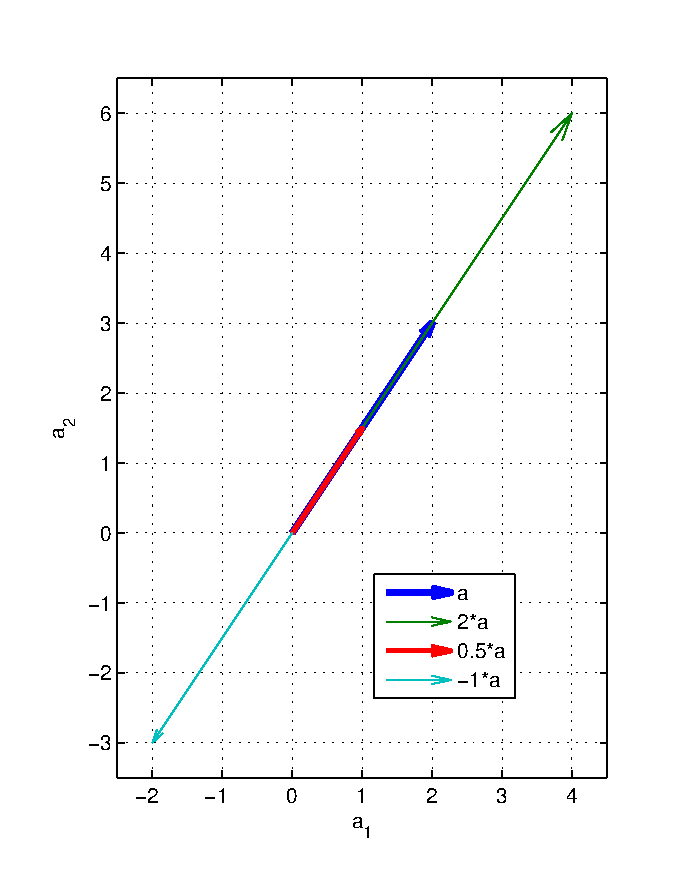
\includegraphics[width=7cm]{vmod.eps}
\caption{efecto del producto de un escalar por un vector}
\label{fig:vmod}
\end{figure}

\paragraph{Combinación lineal.} Combinando la suma de vectores, con el producto por un escalar, podemos generar nuevos vectores, a partir de otros, el proceso se conoce como combinación lineal,
\begin{equation*}
c=\alpha \cdot a + \beta \cdot b + \cdots +\theta z
\end{equation*}

Así el vector $c$ sería el resultado de una combinación  lineal de los vectores $a, b \cdots z$. 
Dado un conjunto de vectores, se dice que son linealmente independientes entre sí, si no es posible poner a unos como combinación lineal de otros,

\begin{equation*}
\alpha \cdot a + \beta \cdot b + \cdots +\theta z=0 \Rightarrow \alpha =\beta =\cdots =\theta =0
\end{equation*}



Es posible expresar cualquier vector de dimensión $n$ como una combinación lineal de $n$ vectores linealmente independientes.

Supongamos $n=2$, cualquier par de vectores que no estén alineados, pueden generar todos los vectores de dimensión $2$ por ejemplo,

\begin{equation*}
\begin{pmatrix}
x_1\\
x_2
\end{pmatrix}=
\alpha \begin{pmatrix}
1\\
2
\end{pmatrix}+\beta \begin{pmatrix}
-1\\
1
\end{pmatrix}
\end{equation*}

La figura \ref{fig:clineal} muestra gráficamente estos dos vectores y algunos de los vectores resultantes de combinarlos linealmente.

\begin{figure}[h]
\centering
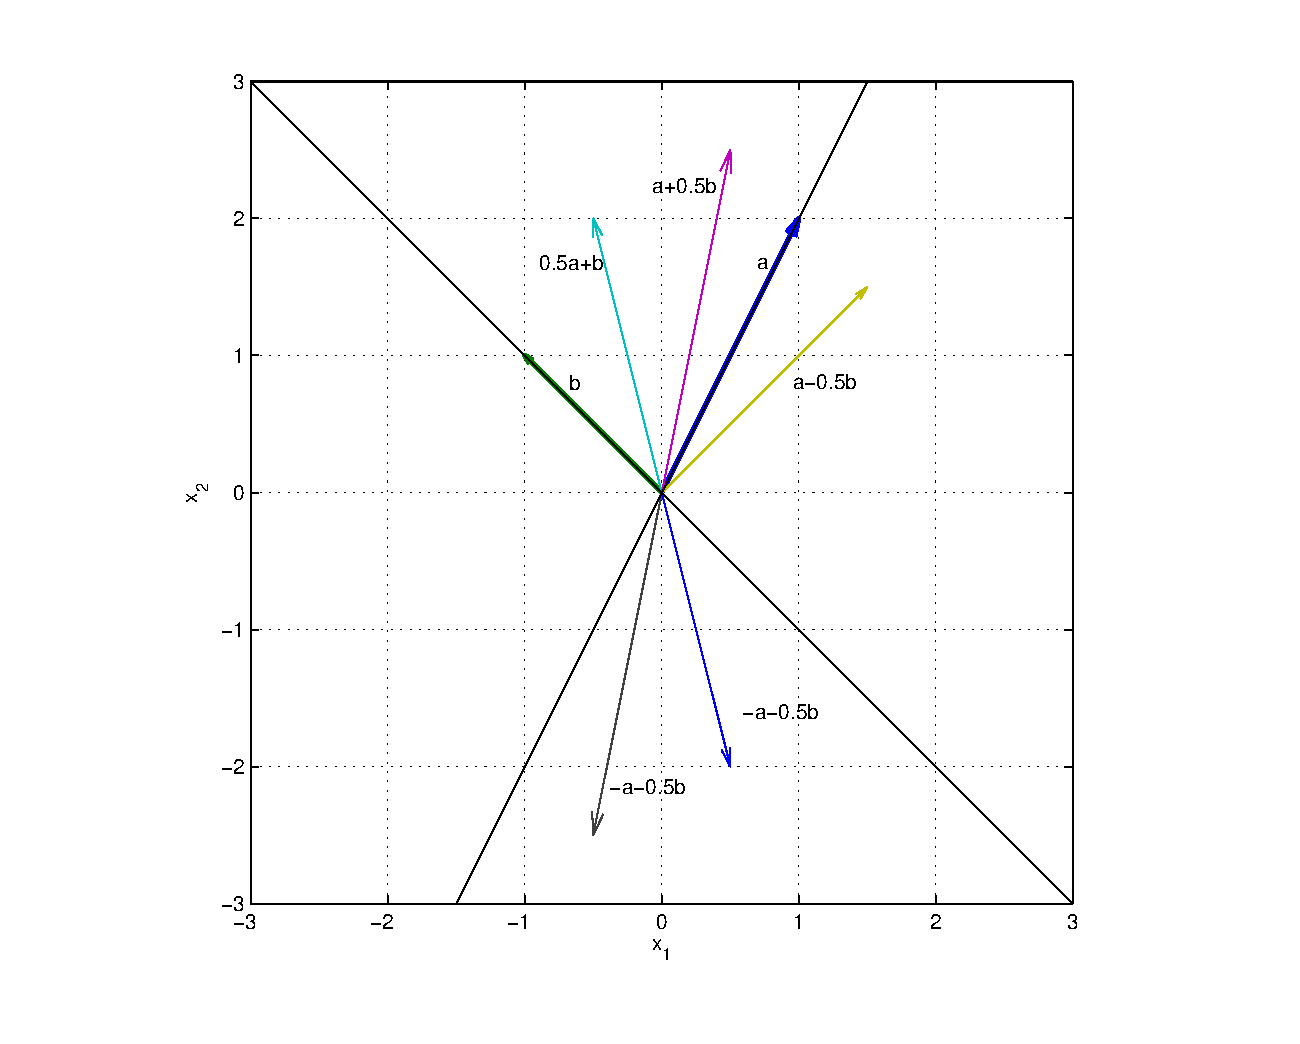
\includegraphics[width=10cm]{clineal.eps}
\caption{Representación gráfica de los vectores $a=(1,2)
$, $b=(-1,1)
$ y algunos vectores, combinación lineal de $a$ y $b$.}
\label{fig:clineal}
\end{figure}
Si tomamos como ejemplo $n=3$, cualquier conjunto de vectores que no estén contenidos en el mismo plano, pueden generar cualquier otro vector de dimensión $3$. Por ejemplo,
\begin{equation*}
\begin{pmatrix}
x_1\\
x_2\\
x_3
\end{pmatrix}=\alpha \begin{pmatrix}
1\\
-2\\
1
\end{pmatrix}+ \beta \begin{pmatrix}
2\\
0\\
-1
\end{pmatrix}+ \gamma \begin{pmatrix}
-1\\
1\\
1
\end{pmatrix}
\end{equation*}

La figura \ref{fig:clin3} muestra gráficamente estos tres vectores y el vector resultante de su combinación lineal, con $\alpha=1$, $\beta=-0.5$ y $\gamma=1$.  Es fácil ver a partir de la figura que cualquier otro vector de dimensión $3$ que queramos construir puede obtenerse a partir de los vectores $a$, $b$ y $c$.
\begin{figure}[h]
\centering
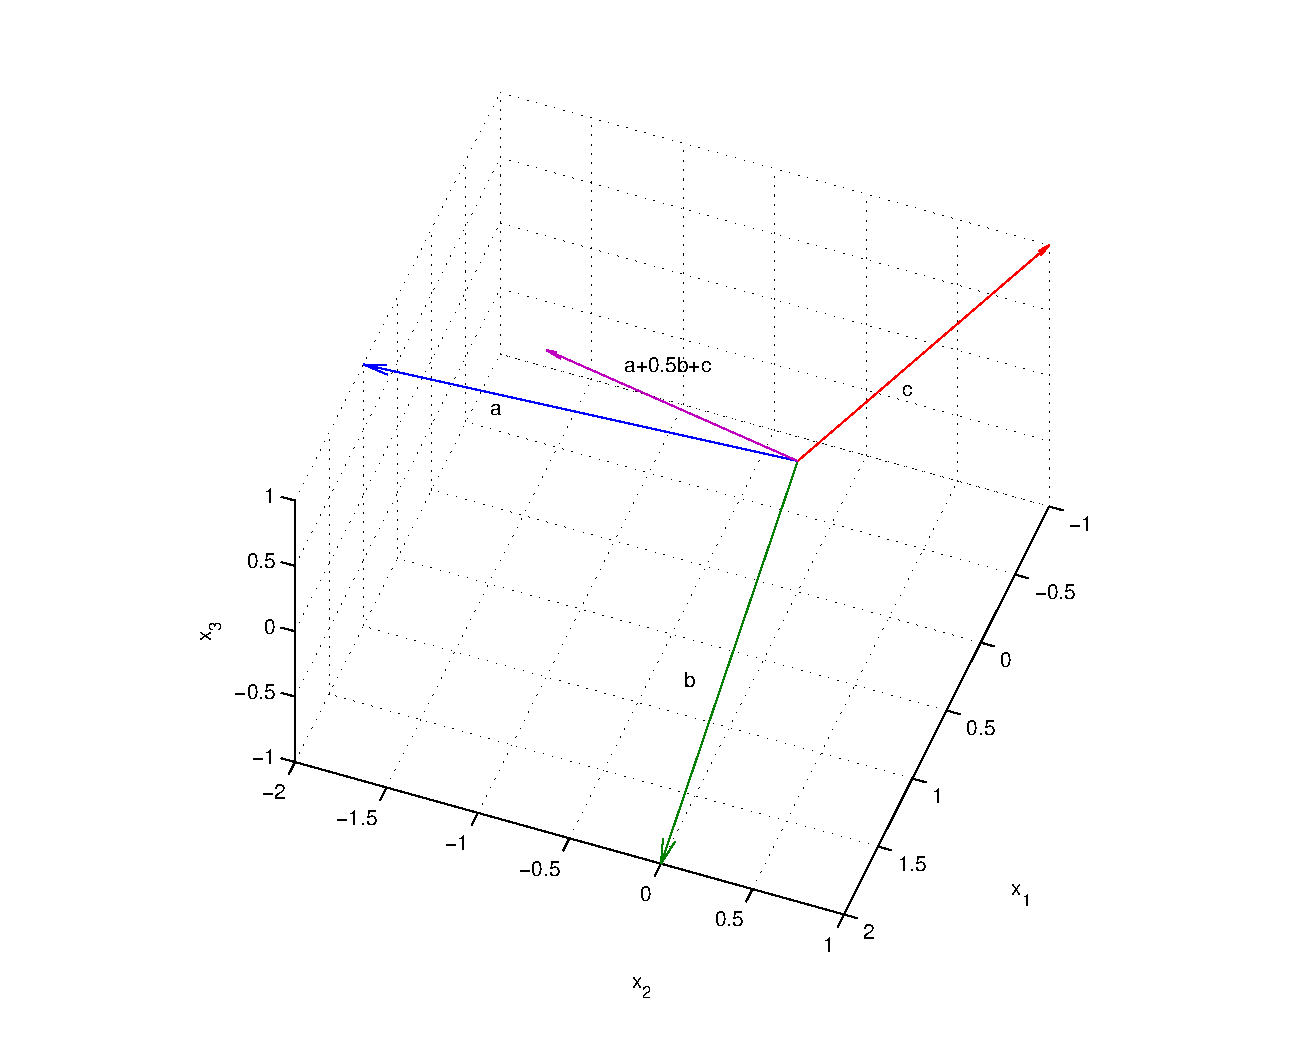
\includegraphics[width=12cm]{clin3.eps}
\caption{Representación gráfica de los vectores $a=(1,-2,1)
$, $b=(2,0,-1)$, $c=(-1,1,1)$ y del vector $a-b+c$.}
\label{fig:clin3}
\end{figure}

\paragraph{Espacio vectorial y  bases del espacio vectorial.} El conjunto de los vectores de dimensión $n$ (matrices de orden $n\times 1$), junto con la suma vectorial y el producto por un escalar, constituye  un  \emph{espacio vectorial} de dimensión $n$.

 Como acabamos de ver, es posible obtener cualquier vector de dicho espacio vectorial a partir de $n$ vectores linealmente independientes del mismo. Un conjunto de $n$ vectores linealmente independientes de un espacio vectorial de dimensión $n$ recibe el nombre de base del espacio vectorial. En principio es posible encontrar infinitas bases distintas para un espacio vectorial de dimensión $n$. Hay algunas particularmente interesantes,
 
 \subparagraph{Bases ortogonales.} Una base ortogonal es aquella en que todos sus vectores son ortogonales entre sí , es decir cumple que su producto escalar es $b^i\cdot b^j=0, i\neq j$. Donde  $b^i$ representa el \emph{i-ésimo} vector de la base, $\mathcal{B}=\left\lbrace b^1, b^2, \cdots, b^n  \right\rbrace $ .
 
 \subparagraph{Bases ortonormales.} Una base ortonormal, es una base ortogonal en la que, además, los vectores de la base tienen módulo $1$. Es decir, $b^i\cdot b^j=0, i\neq j$ y  $b^i\cdot b^j=1, i = j$. Un caso particularmente útil de base ortonormal es la base canónica, formada por los vectores, 
\begin{equation*}
\mathcal{C}=\left\lbrace c^1=\begin{pmatrix}
1\\
0\\
0\\
\vdots \\
0
\end{pmatrix}, c^2=\begin{pmatrix}
0\\
1\\
0\\
\vdots \\
0
\end{pmatrix},
\cdots
c^{n-1}=\begin{pmatrix}
0\\
0\\
\vdots \\
1\\
0
\end{pmatrix},
c^n=\begin{pmatrix}
0\\
0\\
\vdots \\
0\\
1
\end{pmatrix} \right\rbrace
\end{equation*} 

Podemos considerar las componentes de cualquier vector como los coeficientes de la combinación lineal de la base canónica que lo representa,

\begin{equation*}
a=\begin{pmatrix}
a_1\\
a_2\\
\cdots  \\
a_{n-1}\\
a_n
\end{pmatrix} =a_1\cdot \begin{pmatrix}
1\\
0\\
0\\
\vdots \\
0
\end{pmatrix}+a_2 \cdot  \begin{pmatrix}
0\\
1\\
0\\
\vdots \\
0
\end{pmatrix}+
\cdots +
a_{n-1}\cdot \begin{pmatrix}
0\\
0\\
\vdots \\
1\\
0
\end{pmatrix}+
a_n\cdot \begin{pmatrix}
0\\
0\\
\vdots \\
0\\
1
\end{pmatrix}
\end{equation*}

Por extensión, podemos generalizar este resultado a cualquier otra base, es decir podemos agrupar en un vector los coeficientes de la combinación lineal de los vectores de la base que lo generan. Por ejemplo, si construimos, para los vectores de dimensión $3$ la base,
\begin{equation*}
\mathcal{B}=\left\lbrace \begin{pmatrix}
1\\
2\\
0
\end{pmatrix}, \begin{pmatrix}
-1\\
0\\
2
\end{pmatrix}, \begin{pmatrix}
1\\
-1\\
1
\end{pmatrix} \right\rbrace
\end{equation*} 

Podemos entonces representar un vector en la base $\mathcal{B}$ como,
\begin{equation*}
\alpha \cdot \begin{pmatrix}
1\\
2\\
0
\end{pmatrix}+\beta \cdot \begin{pmatrix}
-1\\
0\\
2
\end{pmatrix}+ \gamma \cdot \begin{pmatrix}
1\\
-1\\
1
\end{pmatrix} \rightarrow a^{\mathcal{B}}=\begin{pmatrix}
\alpha \\
\beta \\
\gamma
\end{pmatrix}
\end{equation*} 
 
Donde  estamos empleando el superíndice $^{\mathcal{B}}$, para indicar que las componentes del vector $a$ están definidas con respecto a la base $\mathcal{B}$.

Así por ejemplo el vector,
\begin{equation*}
a^{\mathcal{B}}=\begin{pmatrix}
1.125\\
0.375\\
0.75
\end{pmatrix}
\end{equation*}

Tendría en la base canónica las componentes, 
\begin{equation*}
a^{\mathcal{B}}=\begin{pmatrix}
1.125\\
0.375\\
0.75
\end{pmatrix} \rightarrow a= 1.125 \cdot \begin{pmatrix}
1\\
2\\
0
\end{pmatrix}+0.375 \cdot \begin{pmatrix}
-1\\
0\\
2
\end{pmatrix}+ 0.75 \cdot \begin{pmatrix}
1\\
-1\\
1
\end{pmatrix} =\begin{pmatrix}
1.5\\
1.5 \\
1.5
\end{pmatrix}
\end{equation*}

La figura \ref{fig:base1}, muestra gráficamente la relación entre los vectores de la base canónica $\mathcal{C}$, los vectores de la base $\mathcal{B}$, y el vector $a$, cuyas componentes se han representado en ambas bases.

Podemos aprovechar el producto de matrices para obtener las componentes en la base canónica $\mathcal{C}$ de un vector representado en una base cualquiera $\mathcal{B}$. Si agrupamos los vectores de la base $\mathcal{B}$, en una matriz $B$,

\begin{figure}[h]
\centering
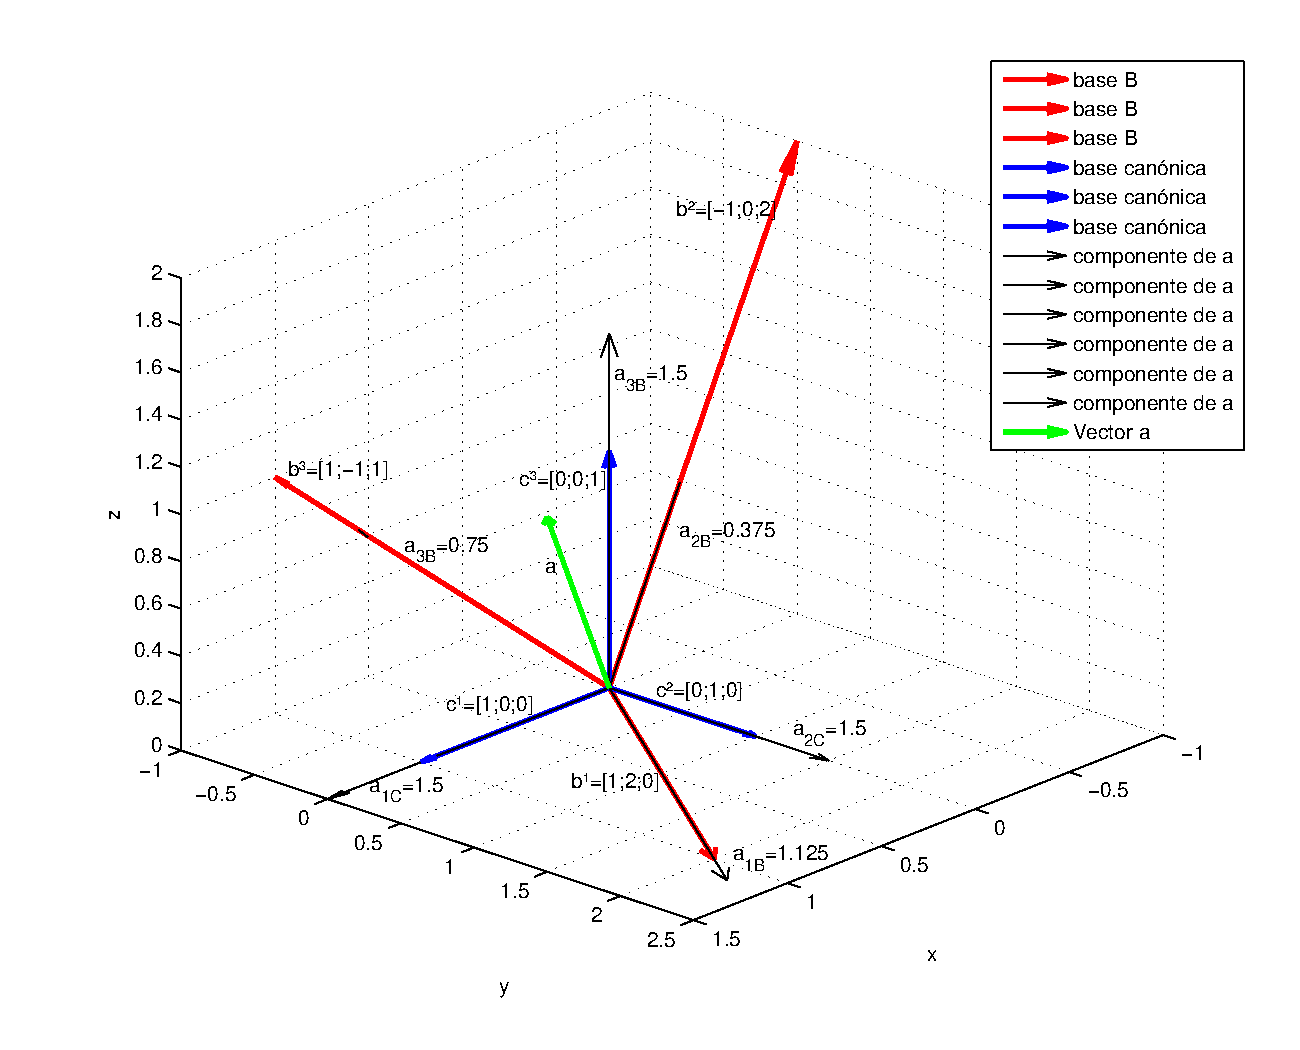
\includegraphics[width=15cm]{base1.eps}
\caption{Representación gráfica del vector $a$, en las base canónica $\mathcal{C}$ y en la base $\mathcal{B}$}
\label{fig:base1}
\end{figure}

\begin{equation*}
\mathcal{B}=\left\lbrace b^1=\begin{pmatrix}
b_{11}\\
b_{21}\\
b_{31}\\
\vdots \\
b_{n1}
\end{pmatrix},b^2=\begin{pmatrix}
b_{12}\\
b_{22}\\
b_{32}\\
\vdots \\
b_{n2}
\end{pmatrix},
\cdots
b^n=\begin{pmatrix}
b_{1n}\\
b_{2n}\\
\vdots \\
b_{(n-1)n}\\
b_{nn}
\end{pmatrix} \right\rbrace \rightarrow
B=\begin{pmatrix}
b_{11}&b_{12}& \cdots & b_{1n}\\
b_{21}&b_{22}& \cdots & b_{2n}\\
b_{31}&b_{32}& \cdots & \vdots \\
\vdots & \vdots & \cdots &  b_{(n-1)n}\\
b_{n1}&b_{n2}& \cdots & b_{nn}\\
\end{pmatrix}
\end{equation*}

Supongamos que tenemos un vector $a$ cuyas componentes en la base $\mathcal{B}$ son,
\begin{equation*}
a^{\mathcal{B}}=\begin{pmatrix}
a_1^{\mathcal{B}}\\
a_2^{\mathcal{B}}\\
\vdots \\
a_n^{\mathcal{B}}
\end{pmatrix}
\end{equation*}

Para obtener las componentes en la base canónica, basta entonces multiplicar la matriz $B$, por el vector $a^{\mathcal{B}}$. Así en el ejemplo que acabamos de ver,

\begin{equation*}
a=B\cdot a^{\mathcal{B}} \rightarrow a=\begin{pmatrix}
1& -1& 1\\
2& 0& -1\\
0& 2& 1
\end{pmatrix}\cdot \begin{pmatrix}
1.125\\
0.375\\
0.75
\end{pmatrix}
= \begin{pmatrix}
1.5\\
1.5\\
1.5
\end{pmatrix}
\end{equation*}

Por último, una podemos combinar el producto de matrices y la matriz inversa, para obtener las componentes de un vector en una base cualquiera a partir de sus componentes en otra base. Supongamos que tenemos dos bases $\mathcal{B}_1$ y $\mathcal{B}_2$ y un vector $a$. Podemos obtener las componentes de $a$ en la base canónica, a partir de las componentes en la base $\mathcal{B}_1$ como, $a=B_1\cdot a^{\mathcal{B}_1}$ y a partir de sus componentes en la base $\mathcal{B}_2$ como $a=B_2\cdot a^{\mathcal{B}_2}$. Haciendo uso de la matriz inversa,

\begin{align*}
a&=B_1\cdot a^{\mathcal{B}_1} \Rightarrow a^{\mathcal{B}_1}=B_1^{-1} \cdot a \\
 a&=B_2\cdot a^{\mathcal{B}_2} \Rightarrow a^{\mathcal{B}_2}=B_2^{-1} \cdot a
\end{align*}

Y sustituyendo obtenemos,

\begin{align*}
a^{\mathcal{B}_1}&=B_1^{-1}\cdot B_2 \cdot a^{\mathcal{B}_2}\\
a^{\mathcal{B}_2}&=B_2^{-1} \cdot B_1\cdot a^{\mathcal{B}_1} 
\end{align*}

El siguiente código permite cambiar de base un vector y representa gráficamente tanto el vector como las bases antigua y nueva.

\begin{verbatim}
function aB2=cambia_vb(aB1,B1,B2)
%este programa cabia de base un vector de dimensión 3 y lo representa en
%relación con las bases antigua y nueva.
%variables de entrada:
%aB1, componentes del vector en la base 1
%B1 base representada como una matriz, (cada columna contiene un vector de
%la base) En la que está representado el vector aB1
%B2, base representada como una matriz, (cada columna contiene un vector de
%la base) en la que se quiere representar el vector aB1
%Si solo se incluye un vector y una base, el programa asume que la segunda
%base es la canonica B2=[1 0 0;0 1 0; 0 0 1]
%variables de salida:
%aB2, Componentes del vector aB1 en la nueva base B2.
%la función hace uso de una función auxiliar (pintavec) incluida al final
%del fichero para dibujar los vectores.

if nargin==2
    %asumimos que queremos cambiar el vector de B1 a la base canonica
    %¿Es B1 una base sensanta?
    if det(B1)<=eps
        error('los vectores de la base no son l. independientes')
    end
    aB2=B1*aB1;
    B2=eye(3); %creamos la base para luego pintarla...
elseif nargin==3
    %cambio de base B1 a B2
    if (det(B1)<=eps)||(det(B2)<=eps)
        error('los vectores de al menos una de las bases no son l. independientes')
    end
    %invertimos la base nueva y multiplicamos por la antigua y por el
    %vector para obtener las componentes del vector en la base nueva.
    aB2=inv(B2)*B1*aB1;
else
    error('el numero de variables de entrada es menor de dos o mayor de tres')
end

%Dibujo de los vectores con la función pintavec....

pintavec(B1,'r') %vectores de la base original
xlabel('x')
ylabel('y')
zlabel('z')
grid on
pintavec(B2,'b') %vectores de la base nueva
for i=1:3
    pintavec(aB1(i)*B1(:,i),'k') %componentes de aB1
    pintavec(aB2(i)*B2(:,i),'k') %componentes de aB2
end
aBc=B1*aB1; %representacion del vector en la base canónica
pintavec(aBc,'g') %vector representado



function pintavec(a,par)
%función auxiliar para pintar vectores... con origen en el origen de
%coordenadas (0,0,0).
%la variable a puede ser un vector o una matriz. y par, es una cadena que contiene los
%típicos parámetros(color, tipo de línea`etc'). El programa considera que
%los vectores están siempre definidos como vectores columnas...
d=size(a,2); %miramos cuantas columnas tiene a, cada columna representará un
%vector distinto
if nargin==2
    for i=1:d
        quiver3(0,0,0,a(1,i),a(2,i),a(3,i),0,par)
        hold on
    end
else
    for i=1:d
        quiver3(0,0,0,a(1,i),a(2,i),a(3,i),0)
    end
end

\end{verbatim}

\paragraph{Operadores lineales.} A partir de los visto en las secciones anteriores, sabemos que el producto de una matriz de $A$ de orden $n\times n$  multiplicada por un vector $b$ de dimension $n$ da como resultado un nuevo vector $c=A\cdot b$  de dimensión $n$. Podemos considerar cada matriz $n\times n$ como un \emph{operador lineal}, que transforma unos vectores en otros.  Decimos que se trata de un operador lineal porque las componentes del vector resultante, están relacionadas linealmente con las del vector original, por ejemplo para $n=3$,
\begin{equation*}
\begin{pmatrix}
y_1\\
y_2\\
y_3
\end{pmatrix}=\begin{pmatrix}
a_{11}& a_{12}& a_{13}\\
a_{21}& a_{22}& a_{23}\\
a_{31}& a_{32}& a_{33}
\end{pmatrix} \cdot
\begin{pmatrix}
x_1\\
x_2\\
x_3
\end{pmatrix} \rightarrow \begin{matrix}
y_1=a_{11}x_1+a_{12}x_2+a_{13}x_3\\
y_2=a_{21}x_1+a_{22}x_2 +a_{23}x_3\\
y_3=a_{31}x_1+a_{32}x_2+a_{33}x_3
\end{matrix} 
\end{equation*}

Entre los operadores lineales, es posible destacar aquellos que producen transformaciones geométricas sencillas. Veamos algunos ejemplos para vectores bidimensionales,

\begin{enumerate}
\item Dilatación: aumenta el módulo de un vector en un factor $\alpha>1$. Contracción: disminuye el módulo de un vector en un factor $0<\alpha<1$. En ambos casos, se conserva la dirección y el sentido del vector original.
 
\begin{equation*}
R=\begin{pmatrix}
\alpha& 0\\
0& \alpha
\end{pmatrix} \rightarrow R\cdot a = \begin{pmatrix}
\alpha& 0\\
0& \alpha
\end{pmatrix} \cdot \begin{pmatrix}
a_1\\
a_2
\end{pmatrix}= \begin{pmatrix}
\alpha \cdot a_1\\
\alpha \cdot a_2
\end{pmatrix}
\end{equation*}

\item Reflexión de un vector respecto al eje x, conservando su módulo,
\begin{equation*}
R_x=\begin{pmatrix}
1& 0\\
0& -1
\end{pmatrix} \rightarrow R_x\cdot a = \begin{pmatrix}
1& 0\\
0& -1
\end{pmatrix} \cdot \begin{pmatrix}
a_1\\
a_2
\end{pmatrix}= \begin{pmatrix}
a_1\\
-a_2
\end{pmatrix}
\end{equation*}

\item Reflexión de un vector respecto al eje y, conservando su módulo,
\begin{equation*}
R_y=\begin{pmatrix}
-1& 0\\
0& 1
\end{pmatrix} \rightarrow R_y\cdot a = \begin{pmatrix}
-1& 0\\
0& 1
\end{pmatrix} \cdot \begin{pmatrix}
a_1\\
a_2
\end{pmatrix}= \begin{pmatrix}
-a_1\\
a_2
\end{pmatrix}
\end{equation*}

\item Reflexión respecto al origen: Invierte el sentido de un vector, conservando su módulo y dirección,
\begin{equation*}
R=\begin{pmatrix}
-1& 0\\
0& -1
\end{pmatrix} \rightarrow R\cdot a = \begin{pmatrix}
-1& 0\\
0& -1
\end{pmatrix} \cdot \begin{pmatrix}
a_1\\
a_2
\end{pmatrix}= \begin{pmatrix}
-a_1\\
-a_2
\end{pmatrix}
\end{equation*}
Sería equivalente a aplicar una reflexión respecto al eje x y luego respecto al eje y o viceversa,
$R=R_x\cdot R_y= R_y\cdot R_x$.

\item Rotación en torno al origen un ángulo $\theta$,
\begin{equation*}
R_{\theta}=\begin{pmatrix}
cos(\theta)& -sin(\theta)\\
sin(\theta)& cos(\theta)
\end{pmatrix} \rightarrow R_{\theta}\cdot a = \begin{pmatrix}
cos(\theta)& -sin(\theta)\\
sin(\theta)& cos(\theta)
\end{pmatrix} \cdot \begin{pmatrix}
a_1\\
a_2
\end{pmatrix}= \begin{pmatrix}
a_1cos(\theta)-a_2sin(\theta)\\
a_1sin(\theta)+a_2cos(\theta)
\end{pmatrix}
\end{equation*}
\end{enumerate}

La figura \ref{fig:ltrans} muestra los vectores resultantes de aplicar las transformaciones lineales que acabamos de describir al vector,  $ a=\bigl( \begin{smallmatrix}
1\\
2
\end{smallmatrix} \bigr)$,

\begin{figure}[h]
\centering
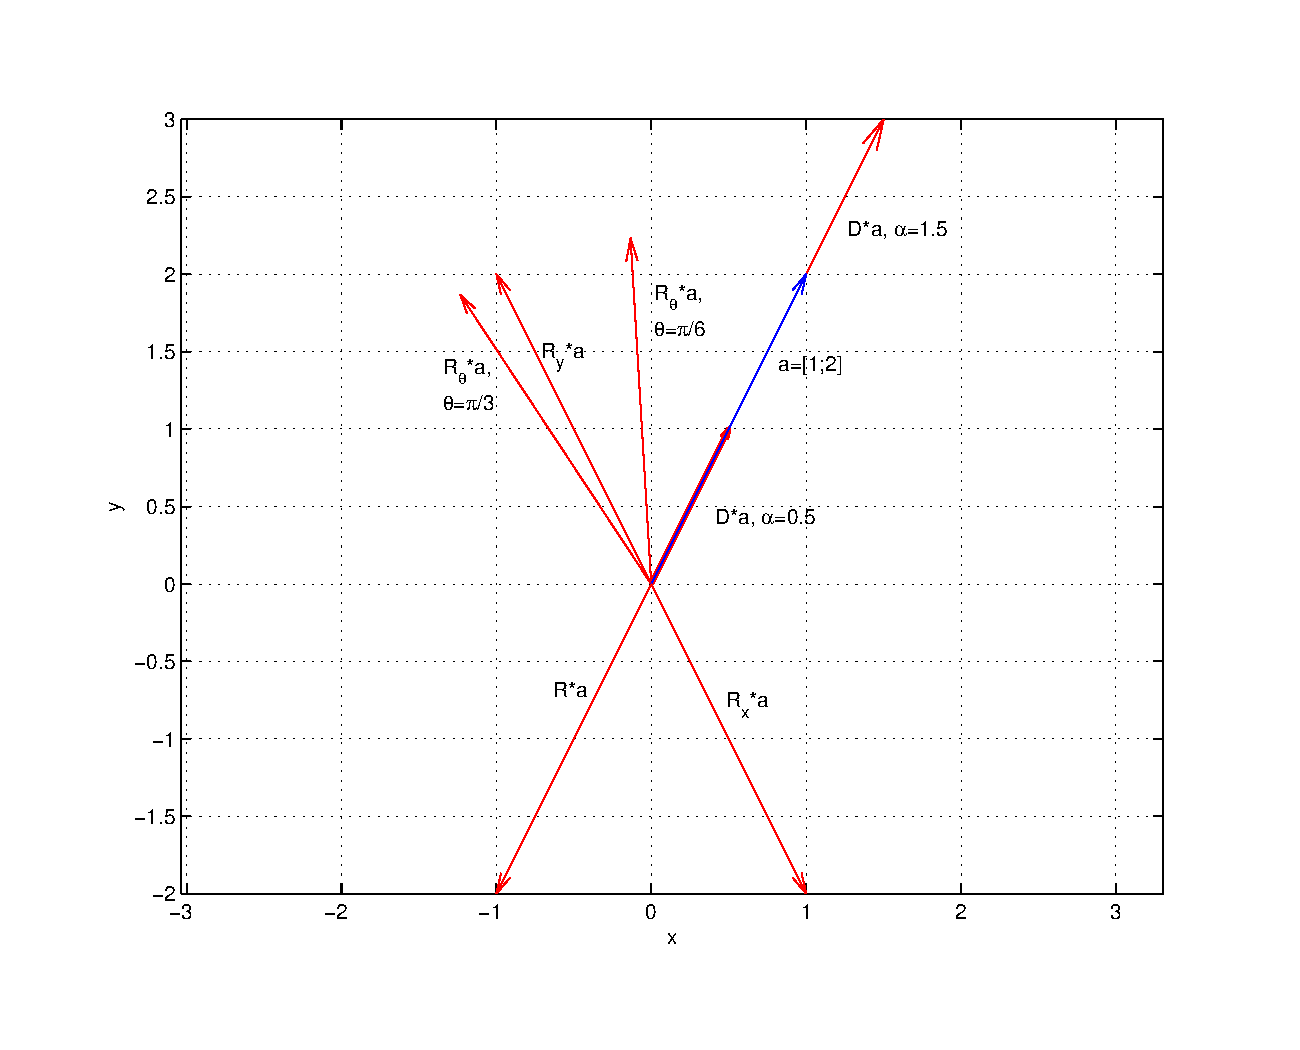
\includegraphics[width=12cm]{ltrans.eps}
\caption{Transformaciones lineales del vector $a=[1;2]$. $D$, dilatación/contracción en un factor $1.5$/$0.5$. $R_x$, reflexión respecto al eje x. $R_y$, reflexión respecto al eje y. $R_{\theta}$ rotaciones respecto al origen para ángulos $\theta=\pi /6$ y $\theta=\pi /3$}
\label{fig:ltrans}
\end{figure}

\paragraph{Norma de una matriz.} La norma de una matriz se puede definir a partir del efecto que produce al actuar, como un operador lineal, sobre un vector. En este caso, se les llama normas \emph{inducidas}. Para una matriz $A$ de orden $m\times n$, $y_{(m)}=A_{(m\times n)}x_{(n)}$, La norma inducida de $A$ se define en función de las normas de los vectores$x$ de su dominio y de las normas de los vectores $y$ de su rango como,
\begin{equation*}
\Vert A \Vert =\max_{x \neq 0} \frac{\Vert y \Vert}{\Vert x \Vert}=\max_{x \neq 0} \frac{\Vert Ax \Vert}{\Vert x \Vert}
\end{equation*}

Se puede interpretar como el factor máximo con que el que la matriz $A$ puede \emph{alargar} un vector cualquiera. Es posible definir la norma inducida en función de los vectores unitarios del dominio,
\begin{equation*}
\Vert A \Vert =\max_{x \neq 0} \frac{\Vert Ax \Vert}{\Vert x \Vert}= \max_{x \neq 0} \left\Vert A\frac{x}{\Vert x \Vert} \right\Vert= \max_{\Vert x \Vert =1}\Vert Ax \Vert
\end{equation*}

Junto a la norma inducida que acabamos de ver, se definen las siguientes normas,

\begin{enumerate}
\item Norma 1: Se suman los elementos de cada columna de la matriz, y se toma coma norma el valor máximo de dichas sumas,
\begin{equation*}
\Vert A_{m,n} \Vert _{1} = \max_j \sum_{i=1}^m a_{ij}
\end{equation*}
 \item Norma $\infty$: Se suman los elementos de cada fila y se toma como norma $\infty$ el valor máximo de dichas sumas.
\begin{equation*}
\Vert A_{m,n} \Vert _{\infty} = \max_i \sum_{j=1}^m a_{ij}
\end{equation*}

\item Norma 2: Se define como el mayor de los valores singulares de una matriz. (Ver sección \ref{sec:SVD}).
\begin{equation*}
\Vert A_{m,n} \Vert _2 = \sigma_{11}
\end{equation*}
\item Norma de Frobenius. Se define como la raíz cuadrada de la suma de los cuadrados de todos los elementos de la matriz,
\begin{equation*}
\Vert A_{m,n} \Vert _F =\sqrt{\sum_{i=1}^m \sum_{j=1}^m a_{ij}^2}
\end{equation*}
Que también puede expresarse de forma mas directa como,
\begin{equation*}
\Vert A_{m,n} \Vert _F =\sqrt{tr(A^T\cdot A)}
\end{equation*}
\end{enumerate}
En Matlab, es posible calcular las distintas normas de una matriz, de modo análogo a como se calculan para el caso de vectores,  mediante el comando \texttt{norm(A,p)}. Donde \texttt{A}, es ahora un a matriz y \texttt{p} especifica el tipo de norma que se quiere calcular. En el caso de una matriz, el parámetro \texttt{p} solo puede tomar los valores, \texttt{1} (norma 1), \texttt{2} (norma 2), \texttt{inf} (norma $\infty$), y \texttt{'fro'} (norma de frobenius). El siguiente ejemplo muestra el cálculo de las normas 1, 2, $\infty$ y de Frobenius de la misma matriz.
\begin{verbatim}
>> A=[1 3 4 5
2 5 6 -3
1 0 4 3]
A =
     1     3     4     5
     2     5     6    -3
     1     0     4     3
>> n1=norm(A,1)
n1 =
    14
>> n2=norm(A,2)
n2 =
     1.022217214669622e+01
>> ninf=norm(A,inf)
ninf =
    16
>> nfro=norm(A,'fro')
nfro =
     1.228820572744451e+01
\end{verbatim} 

\paragraph{Formas cuadráticas.} Se define como forma cuadrática a la siguiente operación entre una matriz cuadrada $A$ de orden $n \times n$ y un vector $x$ de dimensión $n$,
\begin{equation*}
\alpha=x^T\cdot A \cdot x, \ \alpha \in \mathbb{R}
\end{equation*}

El resultado es un escalar. Así por ejemplo,
\begin{equation*}
A=\begin{pmatrix}
1& 2& -1\\
2& 0& 2\\
3& 2& -2
\end{pmatrix}, \ x=\begin{pmatrix}
1\\
2\\
3
\end{pmatrix} \rightarrow \begin{pmatrix}
1& 2& 3
\end{pmatrix} \cdot \begin{pmatrix}
1& 2& -1\\
2& 0& 2\\
3& 2& -2
\end{pmatrix} \cdot \begin{pmatrix}
1\\
2\\
3
\end{pmatrix}= 21
\end{equation*}

Para dimensión $n=2$, 
\begin{equation*}
\alpha =\begin{pmatrix}
x_1& x_2
\end{pmatrix}\cdot \begin{pmatrix}
a_{11}& a_{12}\\
a_{21}& a_{22}
\end{pmatrix}\cdot \begin{pmatrix}
x_1\\
x_2
\end{pmatrix} \rightarrow x_3\equiv \alpha=a_{11}x_1^2+(a_{12}+a_{21})x_1x_2+a_{22}x_2^2
\end{equation*}

Lo que obtenemos, dependiendo de los signos de $a_{11}$ y $a_{12}$, es la ecuación de un paraboloide o un hiperboloide. En la figura \ref{fig:parabol} Se muestra un ejemplo,
\begin{figure}[h]
\centering
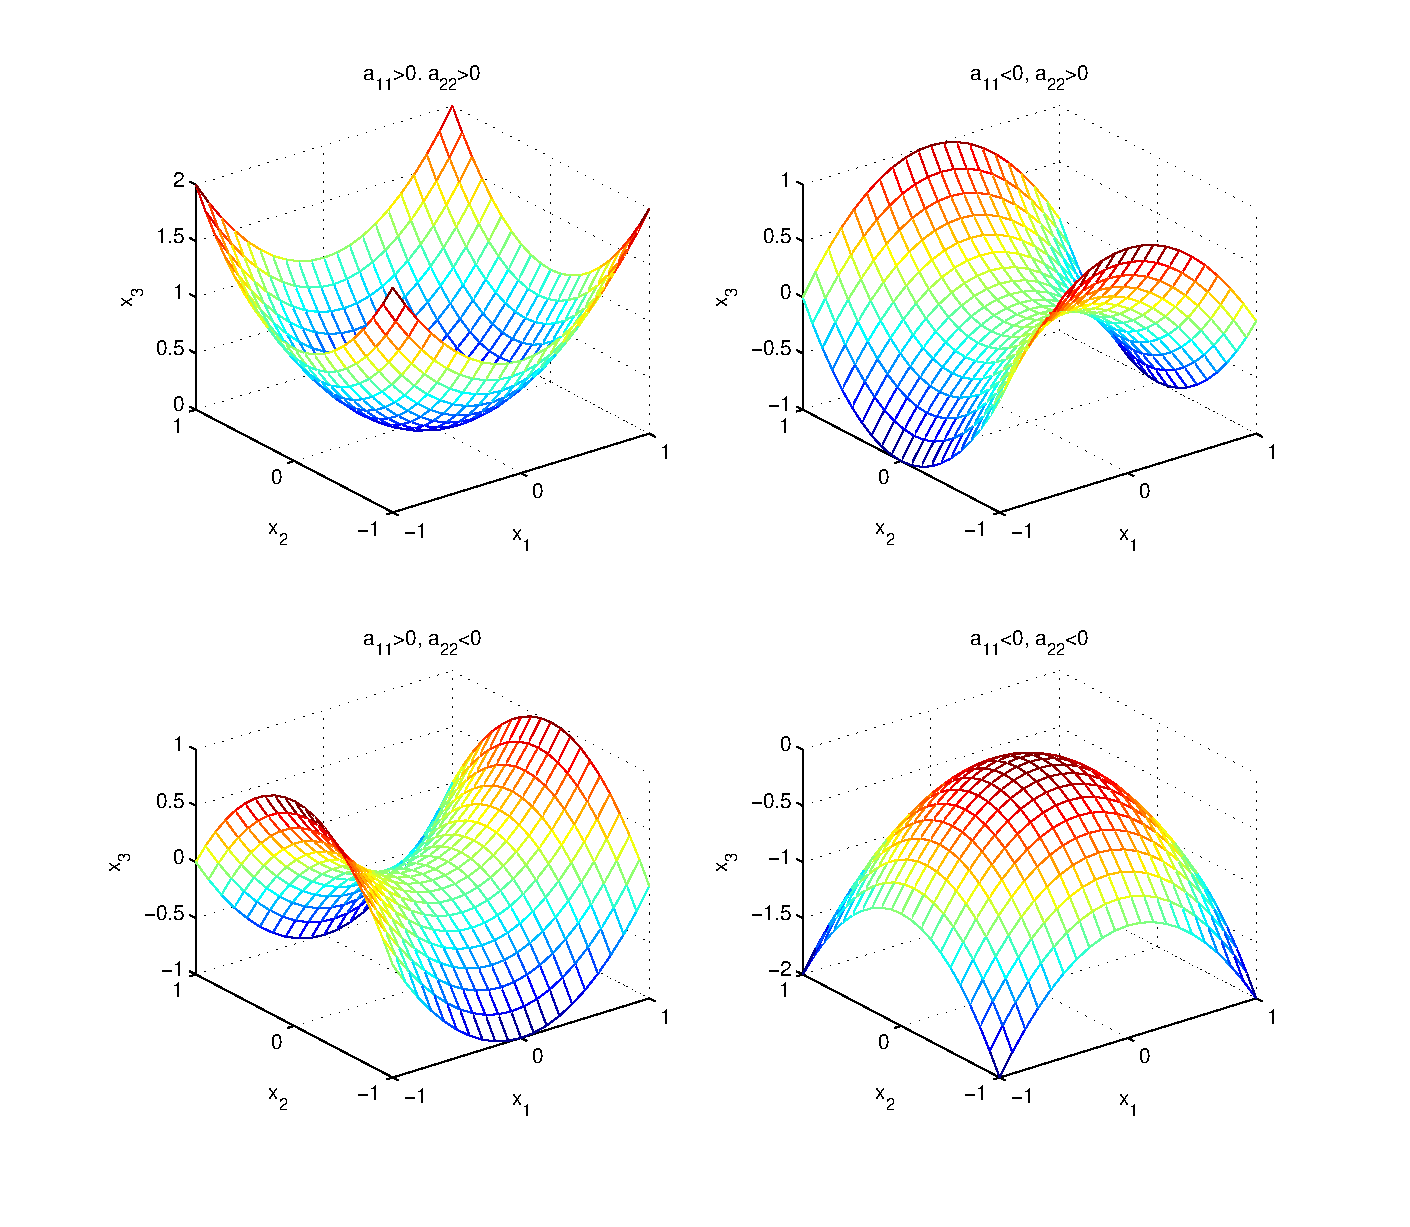
\includegraphics[width=14cm]{parabol.eps}
\caption{Formas cuadráticas asociadas a las cuatro matrices diagonales: $\vert a_{11}\vert=\vert a_{22}\vert=1$, $a_{12}=a_{21}=0$}
\label{fig:parabol}
\end{figure}

Veamos brevemente, algunas propiedades relacionadas con  las formas cuadráticas,
\begin{enumerate}
\item Una matriz $A$ de orden $ n\times n$ se dice que es definida positiva si da lugar a una forma cuadrática que es siempre mayor que cero para cualquier vector no nulo,
\begin{equation*}
x^T \cdot A \cdot x > 0, \forall x \neq 0 
\end{equation*}

\item Una matriz \emph{simétrica} es definida positiva si todos sus \emph{valores propios} (ver sección \ref{sec:diag}) son positivos.

\item Una matriz no simétrica $A$ es definida positiva si su parte simétrica $A_s=(A+A^T)/2$ lo es.
\begin{equation*}
x\cdot A_s\cdot >0, \forall x \neq 0 \Rightarrow x\cdot A\cdot >0, \forall x \neq 0
\end{equation*}
\end{enumerate}

\section{Tipos de matrices empleados frecuentemente}\label{tiposm}
Definimos a continuación algunos tipos de matrices frecuentemente empleados en álgebra, algunos ya han sido introducidos en secciones anteriores. Los reunimos todos aquí para facilitar su consulta

\begin{enumerate}
\item Matriz ortogonal: Una matriz $A_{n\times n}$ es ortogonal cuando su inversa coincide con su traspuesta.
\begin{equation*}
A^T=A^{-1}
\end{equation*}
ejemplo,

\begin{equation*}
A=\begin{pmatrix}
1/3& 2/3& 2/3\\
2/3& -2/3& 1/3\\
2/3& 1/3& -2/3\\
\end{pmatrix} \rightarrow A\cdot A^T =A^T\cdot A= \begin{pmatrix}
1& 0& 0\\
0& 1& 0\\
0& 0& 1
\end{pmatrix}
\end{equation*}
\item Matriz simétrica: Una matriz $A_{n\times n}$ es simétrica cuando es igual que su traspuesta,
\begin{equation*}
A=A^T \rightarrow a_{ij}=a_{ji}
\end{equation*}
ejemplo,
\begin{equation*}
A=\begin{pmatrix}
1& -2& 3\\
-2& 4& 0\\
3& 0& -5
\end{pmatrix}
\end{equation*} 
\item Matriz Diagonal: Una matriz $A$  es diagonal si solo son distintos de ceros los elementos de su diagonal principal,
\begin{equation*}
\begin{pmatrix}
a_{11}& 0& \cdots & 0\\
0& a_{22}& \cdots & 0\\
\vdots & \vdots & \ddots & 0\\
0& 0& \cdots & a_{nn}
\end{pmatrix} \rightarrow
a_{ij}=0,\ \forall i\neq j
\end{equation*}

\item Matriz triangular superior: Una matriz es triangular superior cuando todos los elementos situados por debajo de la diagonal son cero. Es estrictamente diagonal superior si además los elementos de la diagonal también son cero,
\begin{align*}
TRS& \rightarrow a_{ij} = 0, \ \forall i\geq j \\
ETRS& \rightarrow a_{ij} = 0, \ \forall i > j 
\end{align*}
ejemplos,
\begin{align*}
TRS&=\begin{pmatrix}
1 & 3 & 7\\
0 & 2 & -1\\
0 & 0 & 4
\end{pmatrix}\\
ETRS&=\begin{pmatrix}
0 & 3 & 7\\
0 & 0 & -1\\
0 & 0 & 0
\end{pmatrix}\\
\end{align*}
\item Matriz triangular inferior: Una matriz es triangular inferior si todos los elementos pro encima de su diagonal son cero. Es estrictamente triangular inferior si además los elementos de su diagonal son también cero,
\begin{align*}
TRI& \rightarrow a_{ij} = 0, \ \forall i\leq j \\
ETRI& \rightarrow a_{ij} = 0, \ \forall i < j 
\end{align*}
ejemplos,
\begin{align*}
TRI&=\begin{pmatrix}
1 & 0 & 0\\
3 & 2 & 0\\
7 & -1 & 4
\end{pmatrix}\\
ETRI&=\begin{pmatrix}
0 & 0 & 0\\
3 & 0 & 0\\
7 & -1 & 0
\end{pmatrix}\\
\end{align*}
\item Matriz definida Positiva. Una Matriz $A_{n \times n}$ es definida positiva si dado un vector $x$ no nulo cumple,
\begin{equation*}
x^T\cdot A \cdot x > 0, \ \forall x\neq 0
\end{equation*}
si,
\begin{equation*}
x^T\cdot A \cdot x \geq 0, \ \forall x\neq 0
\end{equation*}

entonces la matriz $A$ es semidefinida positiva.

\item Una matriz es Diagonal dominante si cada uno de los elementos de la diagonal en valor absoluto es mayor que la suma de los valores absolutos de los elementos de fila a la  que pertenece.

\begin{equation*}
\lvert a_{ii} \rvert > \sum_{j\neq i} \lvert a_{ij} \rvert, \ \forall i
\end{equation*}
ejemplo,
\begin{equation*}
A=\begin{pmatrix}
10& 2 & 3\\
2& -5 & 1\\
4& -2 & 8
\end{pmatrix}\rightarrow \left\{ \begin{aligned}
10& > 2+3\\
5&> 2+1\\
8& > 4+2
\end{aligned} \right. 
\end{equation*}

\end{enumerate}



\section{Factorización de matrices}\label{sec:fact}
La factorización de matrices, consiste en la descomposición de una matriz en el producto de dos o más matrices. Las matrices resultantes de la factorización se eligen de modo que simplifiquen, o hagan más robustas numéricamente determinadas operaciones matriciales: Cálculos de determinantes, inversas, etc. A continuación se describen las más comunes.

\subsection{Factorizacion LU}\label{sec:LU}
Consiste en factorizar una matriz como el producto de una matriz triangular inferior $L$ por una  matriz triangular superior $U$, $A=L\cdot U$. Por ejemplo,
\begin{equation*}
\begin{pmatrix}
3& 4& 2\\
2& 0& 1\\
3& 2& 1
\end{pmatrix} = \begin{pmatrix}
1& 0& 0\\
^2/_3 & 1& 0\\
1& ^3/_4& 1
\end{pmatrix}\cdot \begin{pmatrix}
3& 4& 2\\
0& ^{-8}/_3& ^{-1}/_3\\
0& 0& ^{-3}/_4
\end{pmatrix}
\end{equation*}
Una aplicación inmediata, es el calculo del determinante. Puesto que el determinante de una matriz triangular, es directamente el producto de los elementos de la diagonal.

En el ejemplo anterior,
\begin{equation*}
\vert A \vert = 6 \equiv \vert L \vert\cdot\vert U\vert =1 \cdot 1 \cdot 1 \cdot 3 \cdot (-\frac{8}{3})\cdot (-\frac{3}{4})=6    
\end{equation*}

Uno de los métodos más conocidos para calcular la factorización LU de una matriz, se basa en el método conocido como eliminación gaussiana. La idea es convertir en ceros los elementos situados por debajo de la diagonal de la matriz. Para ello, se sustituyen progresivamente las filas de la matriz, exceptuando la primera, por combinaciones  formadas con la fila que se sustituye y la fila anterior.
 veamos en qué consiste con un ejemplo. Supongamos que tenemos la siguiente matriz de orden $4 \times 4$, 

\begin{equation*}
A=\begin{pmatrix}
3& 4& 2&5\\
2& 0& 1& -2\\
3& 2& 1& 8\\
5& 2& 3& 2
\end{pmatrix} 
\end{equation*}

Si sustituimos la segunda fila por el resultado de restarle la primera multiplicada por $2$ y dividida por $3$ obtendríamos la matriz,

\begin{equation*}
A=\begin{pmatrix}
3& 4& 2&5\\
2& 0& 1& -2\\
3& 2& 1& 8\\
5& 2& 3& 2
\end{pmatrix} \rightarrow [2\ 0\ 1\ -2]-\frac{2}{3} [3\ 4\ 2\ 5] \rightarrow U_1=\begin{pmatrix}
3& 4& 2&5\\
0& -2.6& -0.33& -5.33\\
3& 2& 1& 8\\
5& 2& 3& 2
\end{pmatrix}
\end{equation*}

De modo análogo, si sustituimos ahora la tercera fila por el resultado de restarle la primera multiplicada por $3$ y dividida $3$,
 
\begin{equation*}
U_1=\begin{pmatrix}
3& 4& 2&5\\
0& -2.6& -0.33& -5.33\\
3& 2& 1& 8\\
5& 2& 3& 2
\end{pmatrix} \rightarrow [3\ 2\ 1\ 8]-\frac{3}{3} [3\ 4\ 2\ 5] \rightarrow U_1=\begin{pmatrix}
3& 4& 2&5\\
0& -2.6& -0.33& -5.33\\
0& -2& -1& -3\\
5& 2& 3& 2
\end{pmatrix}
\end{equation*}

Por último si sustituimos la última fila por el resultado de restarle la primera multiplicada por $5$ y dividida por $3$,

\begin{equation*}
U_1=\begin{pmatrix}
3& 4& 2&5\\
0& -2.6& -0.33& -5.33\\
0& -2& -1& -3\\
5& 2& 3& 2
\end{pmatrix} \rightarrow [5\ 2\ 3\ 2]-\frac{5}{3} [3\ 4\ 2\ 5] \rightarrow U_1=\begin{pmatrix}
3& 4& 2&5\\
0& -2.6& -0.33& -5.33\\
0& -2& -1& -3\\
0& -4,66& -0.33& -6.33
\end{pmatrix}
\end{equation*}

El resultado que hemos obtenido, tras realizar esta transformación , es una nueva matriz $U$ en la que todos los elementos de su primera columna, por debajo de la diagonal, son ceros.

Podemos proceder de modo análogo para \emph{eliminar} ahora los elementos de la segunda columna situados por debajo de la diagonal. Para ellos sustituimos la tercera fila  por la diferencia entre ella y las segunda fila multiplicada por 	$-2$  y dividida por $-2.6$.

\begin{align*}
U_1 &=\begin{pmatrix}
3& 4& 2&5\\
0& -2.6& -0.33& -5.33\\
0& -2& -1& -3\\
0& -4,66& -0.33& -6.33
\end{pmatrix} \rightarrow [0\ -2\ -1\ -3]-\frac{-2}{-2.6} [0\ -2.6\ -0.33\ -5.33\ ] \rightarrow \\
 U_2 &=\begin{pmatrix}
3& 4& 2&5\\
0& -2.6& -0.33& -5.33\\
0& 0& -0.75& 7\\
0& -4.66& -0.33& -6.33
\end{pmatrix}
\end{align*}

Y sustituyendo la última fila por  la diferencia entre ella y la segunda multiplicada por $-4.66$ y dividida por $-2.6$,

\begin{align*}
U_2 &=\begin{pmatrix}
3& 4& 2&5\\
0& -2.6& -0.33& -5.33\\
0& -2& -1& -3\\
0& -4,66& -0.33& -6.33
\end{pmatrix} \rightarrow [0\ -4.66\ -0.33\ -6.33]-\frac{-4.66}{-2.6} [0\ -2.6\ -0.33\ -5.33\ ] \rightarrow \\
 U_2 &=\begin{pmatrix}
3& 4& 2&5\\
0& -2.6& -0.33& -5.33\\
0& 0& -0.75& 7\\
0& 0& 0.25& 3
\end{pmatrix}
\end{align*}

De este modo, los elementos de la segunda columna situados debajo de la diagonal, han sido sustituidos por ceros. Un último paso, nos llevará hasta una matriz triangular superior; sustituimos la última fila por la diferencia entre ella y la tercera fila multiplicada por $0.25$ y dividida por $-0.75$,

\begin{align*}
 U_2 &=\begin{pmatrix}
3& 4& 2&5\\
0& -2.6& -0.33& -5.33\\
0& 0& -0.75& 7\\
0& 0& 0.25& 3
\end{pmatrix} \rightarrow [0\ 0\ 0.25\ 3]-\frac{0.25}{-0.75} [0\ 0\ -0.75\ 7\ ] \rightarrow \\
 U_3 &=\begin{pmatrix}
3& 4& 2&5\\
0& -2.6& -0.33& -5.33\\
0& 0& -0.75& 7\\
0& 0& 0& 5.33
\end{pmatrix}=U
\end{align*}

Podemos ahora, a partir del ejemplo, deducir un procedimiento general. Para \emph{eliminar} ---convertir en 0--- el elemento $a_{ij}$ situado por debajo de la diagonal principal,  $i>j$:
\begin{enumerate}
\item Dividimos los elementos de la fila $j$ por el elemento de dicha fila que a su vez pertenece a la diagonal, $a_{jj}$
\begin{equation*}
\begin{bmatrix}
0/ a_{jj}& 0/ a_{jj}& \cdots & a_{jj}/ a_{jj}& a_{jj+1}/ a_{jj}& \cdots
\end{bmatrix}
\end{equation*}

\item Multiplicamos el resultado de la operación anterior por el elemento $a_{ij}$,
\begin{equation*}
\begin{bmatrix}
a_{ij} \cdot 0/ a_{jj}& a_{ij} \cdot 0/ a_{jj}& \cdots & a_{ij} \cdot a_{jj}/ a_{jj}& a_{ij} \cdot a_{jj+1}/ a_{jj}& \cdots
\end{bmatrix}
\end{equation*}
\item Finalmente, sustituimos la fila $i$ de la matriz de partida por la diferencia  entre ella y el resultado de la operación anterior.
\begin{equation*}
\begin{bmatrix}
0& 0& \cdots& a_{ij}& a_{ij+1}& \cdots
\end{bmatrix}-\begin{bmatrix}
a_{ij} \cdot 0/ a_{jj}& a_{ij} \cdot 0/ a_{jj}& \cdots & a_{ij} \cdot a_{jj}/ a_{jj}& a_{ij} \cdot a_{jj+1}/ a_{jj}& \cdots
\end{bmatrix}
\end{equation*}
\end{enumerate}

Este procedimiento se aplica iterativamente empezando en por el elemento  $a_{21}$ de la matriz y desplazando el cómputo hacia abajo, hasta llegar a la última fila y hacia la derecha hasta llegar en cada fila al elemento anterior a la diagonal.

El siguiente código aplica el procedimiento descrito a una matriz de cualquier orden,\label{elig}

\begin{verbatim}
function U=eligauss(A)
%Esta función obtiene una matriz triangular superior, a partir de una
%matriz dada, aplicando el método de eliminación gaussiana.
%No realiza piboteo de filas, así que si algún elemento de la diagonal de A
%queda cero o proximo a cero al ir eliminado dará problemas...

%Obtenemos el número de filas de la matriz..
nf=size(A,1);
U=A
%
for j=1:nf-1 %recorro todas la columnas menos la última
    for i=j+1:nf %Recorro las filas desde debajo de la diagonal hasta la última
        %en Matlab tengo la suerte de poder manejar cada fila de un solo
        %golpe.
        U(i,:)=U(i,:)-U(j,:)*U(i,j)/U(j,j)
    end
end

\end{verbatim}

Hasta ahora, hemos descrito un procedimiento para transformar una matriz cualquiera en una matriz triangular superior. Nuestro objetivo era obtener la descomposición de un matriz en el producto de dos,  una triangular inferior y otra triangular superior.  En primer lugar, podemos asociar    el procedimiento descrito de eliminación gaussiana al producto de matrices. Volviendo al ejemplo anterior, si construimos la matriz $\lambda_1$
\begin{equation*}
\lambda_1=\begin{pmatrix} 
1& 0& 0& 0\\
-2/3& 1& 0& 0\\
-3/3& 0& 1& 0\\
-5/3& 0& 0& 1
\end{pmatrix}
\end{equation*},
El producto $\lambda_1 \cdot A$ da como resultado la matriz,

\begin{equation*} 
 U_1=\begin{pmatrix}
3& 4& 2&5\\
0& -2.66& -0.33& -5.33\\
0& -2& -1& -3\\
0& -4.66& -0.33& -6.33
\end{pmatrix}=\begin{pmatrix} 
1& 0& 0& 0\\
-2/3& 1& 0& 0\\
-3/3& 0& 1& 0\\
-5/3& 0& 0& 1
\end{pmatrix}\cdot \begin{pmatrix}
3& 4& 2&5\\
2& 0& 1& -2\\
3& 2& 1& 8\\
5& 2& 3& 2
\end{pmatrix}
\end{equation*}

De modo análogo, $U_2=\lambda_2 \cdot U_1$
 
\begin{equation*}
\lambda_2=\begin{pmatrix} 
1& 0& 0& 0\\
0& 1& 0& 0\\
0& -2/2.66& 1& 0\\
0& -4.66/2.66& 0& 1
\end{pmatrix}
\end{equation*}

\begin{equation*}
U_2= \begin{pmatrix}
3& 4& 2&5\\
0& -2.6& -0.33& -5.33\\
0& 0& -0.75& 7\\
0& 0& 0.25& 3
\end{pmatrix}
\end{equation*}

Por último, $U=\lambda_3 \cdot U_2$

\begin{equation*}
 \lambda_3 =\begin{pmatrix}
1& 0& 0&0\\
0& 1& 0& 0\\
0& 0& 1& 0\\
0& 0& 0.25/0.75 & 1
\end{pmatrix}
\end{equation*}

\begin{equation*}
 U =\begin{pmatrix}
3& 4& 2&5\\
0& -2.66& -0.33& -5.33\\
0& 0& -0.75& 7\\
0& 0& 0& 5.33
\end{pmatrix}
\end{equation*}

De nuevo, podemos generalizar el procedimiento empleado; cada matriz $\lambda_j$ \emph{elimina} todos los elementos de la columna $n$ de una matriz $A$ , situados por debajo de la diagonal. La  matriz $\lambda_j$  toma la forma general,

\begin{equation*}
\lambda_j=\begin{pmatrix}
1& \cdots & 0& 0& 0& \cdots & 0\\
 \vdots &  &  \vdots & \vdots &  \vdots & & \vdots\\
0& \cdots & 1& 0& 0& \cdots & 0\\
0& \cdots & 0& 1& 0& \cdots & 0\\
0& \cdots &0 & -a_{j+1,j}/a_{jj}& 0& \cdots & 0\\
0& \cdots &0 & -a_{j+2,j}/a_{jj}& 1& \cdots & 0\\
 \vdots &  &  \vdots & \vdots &  \vdots & & \vdots\\
0& \cdots & 0& -a_{n,j}/a_{jj}& 0&\cdots & 1\\
\end{pmatrix}
\end{equation*} 
Solo los elementos de la diagonal, que toman el valor $1$, y los elementos de la columna $j$ situados por debajo de la diagonal son distintos de cero.

A partir de la definición de las matrices $\lambda_j$, podemos obtener una relación entre la matriz triangular superior $U$  obtenida al final del proceso de eliminación, y la matriz inicial $A$ de orden $n\times n$ para ello, en cada paso multiplicamos tanto por $\lambda_j$ como por su inversa $\lambda_j^{-1}$,
\begin{align*}
A&=\lambda_1^{-1}\cdot \overbrace{\lambda_1\cdot A}^{U_1}\\
A&=\lambda_1^{-1}\cdot\lambda_2^{-1} \cdot \overbrace{\lambda_2  \cdot \lambda_1 A}^{U_2}\\
A&=\lambda_1^{-1}\cdot \lambda_2^{-1}\cdot \overbrace{ \lambda_3^{-1}\cdot  \lambda_3 \cdot  \lambda_2\cdot \lambda_1 \cdot A}^{U_3}\\
\vdots \\
A&=\lambda_1^{-1} \cdot  \lambda_2^{-1}\cdot  \lambda_3^{-1} \cdots  \lambda_n ^{-1}\cdot \overbrace{\lambda_n \cdots \lambda_3 \cdot \lambda_2\cdot \lambda_1  \cdot A}^{U}
\end{align*}

Las matrices $\lambda_j^{-1}$ tienen dos propiedades que las hacen particularmente fáciles de manejar:  la primera es que cumplen que  su inversa  $\lambda_j^{-1}$ puede obtenerse a partir de $\lambda_j$, sin más que cambiar de signo los elementos distintos de cero que no pertenecen a la diagonal (Compruébalo),
\begin{equation*}
 \lambda_j^{-1}=\begin{pmatrix}
1& \cdots & 0& 0& 0& \cdots & 0\\
 \vdots &  &  \vdots & \vdots &  \vdots & & \vdots\\
0& \cdots & 1& 0& 0& \cdots & 0\\
0& \cdots & 0& 1& 0& \cdots & 0\\
0& \cdots &0 & a_{j+1j}/a_{jj}& 0& \cdots & 0\\
0& \cdots &0 & a_{j+2j}/a_{jj}& 1& \cdots & 0\\
 \vdots &  &  \vdots & \vdots &  \vdots & & \vdots\\
0& \cdots & 0& a_{nj}/a_{jj}& 0&\cdots & 1\\
\end{pmatrix}
\end{equation*}

La segunda propiedad es que el producto $L=\lambda_1^{-1} \cdot  \lambda_2^{-1}\cdot  \lambda_3^{-1} \cdots  \lambda_n ^{-1}$, se puede obtener progresivamente, a la vez que se construye $U$, sin más que ir juntando en una única matriz $L$ las columnas de $\lambda_1^{-1}$, $\lambda_2^{-1}$, etc. que contienen elementos no nulos, en nuestro ejemplo,
\begin{equation*}
 L =\begin{pmatrix}
1& 0& 0&0\\
2/3& 1& 0& 0\\
3/3& 2/2.66& 1& 0\\
5/3& 4.66/2.66& -0.25/0.75 & 1
\end{pmatrix}
\end{equation*}

y, en general,

\begin{equation*}
 L=\begin{pmatrix}
1& \cdots & 0& 0& 0& \cdots & 0\\
 \vdots &  &  \vdots & \vdots &  \vdots & & \vdots\\
a_{j-11}/a_{11}& \cdots & 1& 0& 0& \cdots & 0\\
a_{j1}/a_{11}& \cdots & a_{jj-1}/a_{j-1 j-1}& 1& 0& \cdots & 0\\
a_{j+11}/a_{11}& \cdots &a_{j+1j-1}/a_{j-1 j-1} & a_{j+1j}/a_{jj}& 0& \cdots & 0\\
a_{j+11}/a_{11}& \cdots &a_{j+2j-1}/a_{j-1 j-1} & a_{j+2j}/a_{jj}& 1& \cdots & 0\\
 \vdots &  &  \vdots & \vdots &  \vdots & & \vdots\\
a_{n1}/a_{11}& \cdots & a_{nj-1}/a_{j-1j-1}& a_{nj}/a_{jj}& a_{nj+1}/a_{j+1j+1}&\cdots & 1\\
\end{pmatrix}
\end{equation*}

Por construcción,  la matriz $L$ es una matriz inferior, Con lo que quedaría completo el cálculo de la factorización LU,

\begin{equation*}
A=\overbrace{\lambda_1^{-1} \cdot  \lambda_2^{-1}\cdot  \lambda_3^{-1} \cdots  \lambda_n ^{-1}}^{L}\cdot \overbrace{\lambda_n \cdots \lambda_3 \cdot \lambda_2\cdot \lambda_1  \cdot A}^{U}=L\cdot U
\end{equation*}

La factorización que acabamos de describir, puede presentar problemas numéricos dependiendo del cómo sea la matriz que se desea factorizar. El primer problema se produce cuando el elemento de la diagonal de $u_{jj}$ por el que toca dividir para eliminar los elementos de la columna $j$, situados por debajo de la diagonal, es $0$. En ese caso el ordenador dará un error de desbordamiento y no se podrá seguir factorizando. El segundo problema surge cuando los elementos de la matriz son dispares en magnitud; las operaciones matemáticas realizadas durante el proceso de factorización pueden dar lugar a errores de redondeo importantes que hagan incorrecto el resultado de la factorización. Veamos un ejemplo un tanto extremo,

\begin{equation*}
\begin{pmatrix}
10^{-20}& 1\\
1& 1 
\end{pmatrix}=\overbrace{\begin{pmatrix}
1& 0\\
10^{20}& 1 
\end{pmatrix}}^{L}\cdot \overbrace{\begin{pmatrix}
1& 0\\
-10^{20}& 1
\end{pmatrix}\cdot \begin{pmatrix}
10^{-20}& 1\\
1& 1
\end{pmatrix}}^{U}= \overbrace{\begin{pmatrix}
1& 0\\
10^{20}& 1 
\end{pmatrix}}^{L} \cdot \overbrace{\begin{pmatrix}
10^{-20}& 1\\
0& 1 -10^{20} 
\end{pmatrix}}^{U} 
\end{equation*} 

Como el \emph{eps} del ordenador es del orden de $10^{-16}$, $1$ es despreciado frente $10^{20}$. Es decir, $(1-10^{20})\approx 10^{20}$, con lo cual el ordenador tendrá una versión aproximada de $U$

\begin{equation*}
U \approx \hat{U}= \begin{pmatrix}
10^{-20}& 1\\
0& -10^{20} 
\end{pmatrix} 
\end{equation*}

Pero si ahora volvemos a multiplicar $L\cdot U$  para recuperar $A$,
\begin{equation*}
L \cdot \hat{U}=  \begin{pmatrix}
1& 0\\
10^{20}& 1 
\end{pmatrix} \cdot \begin{pmatrix}
10^{-20}& 1\\
0& -10^{20} 
\end{pmatrix}= \begin{pmatrix}
10^{-20}& 1\\
1& 0
\end{pmatrix} \neq A
\end{equation*}

Una manera de paliar los efectos de redondeo, es reordenar las filas de la matriz de modo que el elemento $a_{jj}$ por el que se va a dividir los elementos de la fila $j$ en el proceso de eliminación sea lo mayor posible. Este procedimiento se conoce con el nombre de pivoteo de filas.
Para el ejemplo que acabamos de examinar, supongamos que cambiamos de orden las dos filas de    la matriz,

\begin{equation*}
\begin{pmatrix}
10^{-20}& 1\\
1& 1 
\end{pmatrix} \rightarrow \begin{pmatrix}
1& 1\\
10^{-20}& 1 
\end{pmatrix}
\end{equation*}

Si recalculamos la factorización LU, para la nueva matriz con la filas intercambiadas,

\begin{equation*}
\begin{pmatrix}
1& 1\\
10^{-20}& 1 
\end{pmatrix}=\overbrace{\begin{pmatrix}
1& 0\\
10^{-20}& 1 
\end{pmatrix}}^{L}\cdot \overbrace{\begin{pmatrix}
1& 0\\
-10^{-20}& 1
\end{pmatrix}\cdot \begin{pmatrix}
1& 1\\
10^{-20}& 1 
\end{pmatrix}}^{U}= \overbrace{\begin{pmatrix}
1& 0\\
10^{-20}& 1 
\end{pmatrix}}^{L} \cdot \overbrace{\begin{pmatrix}
1& 1\\
0&  1-10^{-20}
\end{pmatrix}}^{U} 
\end{equation*}

De nuevo, por errores de redondeo el ordenador tendrá una version aproximada de $U$.

\begin{equation*}
U \approx \hat{U}= \begin{pmatrix}
1& 1\\
0& 1 
\end{pmatrix} 
\end{equation*}

Sin embargo si recalculamos el producto $L\cdot \hat{U}$ y volvemos a reordenar las filas del resultado,
\begin{equation*}
L \cdot \hat{U}=  \begin{pmatrix}
1& 0\\
10^{-20}& 1 
\end{pmatrix} \cdot \begin{pmatrix}
1& 1\\
0& 1 
\end{pmatrix}= \begin{pmatrix}
1& 1\\
10^{-20}& 1+10^{-20}
\end{pmatrix} \rightarrow \begin{pmatrix}
10^{-20}& 1+10^{-20}\\
1& 1
\end{pmatrix} \approx A
\end{equation*}

La permutación de las filas de una matriz $A$ de orden $n\times m$, se puede definir a partir del producto con las matrices de permutación de orden $n \times n$. Éstas se obtienen permutando directamente las filas de la matriz identidad $I_{n \times n}$. Si una matriz de permutación multiplica a otra matriz por la izquierda, permuta el orden de sus filas. Si la multiplica por la derecha. permuta el orden de sus columnas. Así por ejemplo, para matrices de orden $3 \times n$,

\begin{equation*}
I_{n \times n}=\begin{pmatrix}
1& 0& 0\\
0& 1& 0\\
0& 0& 1\\
\end{pmatrix} \rightarrow P_{1 \leftrightarrow 3}= \begin{pmatrix}
0& 0& 1\\
0& 1& 0\\
1& 0& 0\\
\end{pmatrix}
\end{equation*}

Si multiplicamos $P_{1 \leftrightarrow 3}$ con cualquier otra matriz $A$ de orden $3\times n$, El resultado es equivalente a intercambiar en la matriz $A$ la fila $1$ con la $3$. Por ejemplo
   
\begin{equation*}
P_{1\leftrightarrow 3}\cdot A=\begin{pmatrix}
0& 0& 1\\
0& 1& 0\\
1& 0& 0\\
\end{pmatrix} \cdot \begin{pmatrix}
1& 2& 5& 3\\
4& 2& 3& 0\\
3& 6& 2& 1
\end{pmatrix} = \begin{pmatrix}
3& 6& 2& 1\\
4& 2& 3& 0\\
1& 2& 5& 3
\end{pmatrix}= A_{1\leftrightarrow 3}
\end{equation*}

Volvamos al cálculo de la factorización LU, pero ahora empleando pivoteo de filas. Supongamos una matriz $A$ de orden $n\times n$

El primer paso, es buscar el elemento mayor en valor absoluto de la primera columna en intercambia la primera fila de la matriz de $A$, con la fila que contiene dicho elemento. Si utilizamos la matriz de permutación adecuada, esto puede expresarse como,

\begin{equation*}
A \rightarrow P_1\cdot A
\end{equation*}
A continuación eliminamos los elementos de la primera fila situados por debajo de la diagonal,
\begin{equation*}
A \rightarrow P_1\cdot A \rightarrow \lambda_1 \cdot P_1 \cdot A
\end{equation*}
Volvemos a buscar el mayor elemento en valor absoluto para la segunda columna (Solo desde la diagonal hasta el ultimo elemento de la columna).  
\begin{equation*}
A \rightarrow P_1\cdot A \rightarrow \lambda_1 \cdot P_1 \cdot A \rightarrow  P_2 \cdot \lambda_1 \cdot P_1 \cdot A 
\end{equation*}

Eliminamos los elementos de la segunda fila situados por debajo de la diagonal,

\begin{equation*}
A \rightarrow P_1\cdot A \rightarrow \lambda_1 \cdot P_1 \cdot A \rightarrow  P_2 \cdot \lambda_1 \cdot P_1 \cdot A \rightarrow \lambda_2 \cdot  P_2 \cdot \lambda_1 \cdot P_1 \cdot A
\end{equation*}

Si seguimos todo el proceso hasta eliminar los elementos situados por debajo de la diagonal en la fila $n-1$, obtendremos la expresión de la matriz triangular superior $U$ resultante,

\begin{equation*}
\lambda_{n-1}P_{n-1}\lambda_{n-2}P_{n-2} \cdots  \lambda_2  P_2 \lambda_1  P_1 A = U
\end{equation*}

Aunque hemos obtenido $U$, necesitamos una manera de obtener $L$, ahora no es inmediato como en el caso de la factorización sin pivoteo, no basta con invertir las matrices $\lambda_i$ ya que tenemos por medio todas las matrices de permutación utilizadas. Para obtenerla realizaremos la siguiente transformación, 

\begin{equation*}
\lambda_{n-1}P_{n-1}\lambda_{n-2}P_{n-2} \cdots  \lambda_2  P_2 \lambda_1  P_1 A = \lambda_{n-1}'\lambda_{n-2}'\cdots \lambda_2'   \lambda_1' P_{n-1}P_{n-2} \cdots P_2  P_1 A
\end{equation*}

Donde las matrices $\lambda_i'$ pueden obtenerse a partir de las matrices $\lambda_i$ y de las matrices de permutación de la manera siguiente,

\begin{align*}
\lambda_{n-1}' &= \lambda_{n-1} \\
\lambda_{n-2}' &= P_{n-1}\lambda_{n-2} P_{n-1} ^{-1}\\
\lambda_{n-3}' &= P_{n-1}P_{n-2}\lambda_{n-3}P_{n-2}^{-1} P_{n-1}^{-1} \\
 & \vdots \\
 \lambda_{k\ \ }'  &= P_{n-1}P_{n-2}\cdots P_{k+1} \lambda_{k}P_{k+1}^{-1} \cdots P_{n-2}^{1} P_{n-1}^{-1} \\
 & \vdots \\
\lambda_{2\ \ }'  &= P_{n-1}P_{n-2}\cdots P_3 \lambda_{2}P_3^{-1} \cdots P_{n-2}^{1} P_{n-1}^{-1} \\
\lambda_{1\ \ }'  &= P_{n-1}P_{n-2}\cdots P_3P_2 \lambda_{1}P_2^{-1}P_3^{-1} \cdots P_{n-2}^{1} P_{n-1}^{-1} \\
\end{align*}


Matemáticamente el cálculo de las matrices $\lambda_i'$ requiere calcular el producto de un gran número de matrices.  Sin embargo dicho cálculo es equivalente a permutar los elementos de $\lambda_i$ situados por debajo de la diagonal.   Así Por ejemplo para,

\begin{equation*}
\lambda_2=
\begin{pmatrix}
1& 0& 0& 0\\
0& 1& 0& 0\\
0& 2& 1& 0\\
0& 3& 0& 1
\end{pmatrix}, \ 
P_3=
\begin{pmatrix}
1& 0& 0& 0\\
0& 1& 0& 0\\
0& 0& 0& 1\\
0& 0& 1& 0
\end{pmatrix}
\end{equation*}

\begin{equation*}
\lambda_2'=P_3\cdot \lambda_2 P_3^{-1}
\begin{pmatrix}
1& 0& 0& 0\\
0& 1& 0& 0\\
0& 0& 0& 1\\
0& 0& 1& 0
\end{pmatrix}\cdot \begin{pmatrix}
1& 0& 0& 0\\
0& 1& 0& 0\\
0& 2& 1& 0\\
0& 3& 0& 1
\end{pmatrix} \cdot \begin{pmatrix}
1& 0& 0& 0\\
0& 1& 0& 0\\
0& 0& 0& 1\\
0& 0& 1& 0
\end{pmatrix} = \begin{pmatrix}
1& 0& 0& 0\\
0& 1& 0& 0\\
0& 3& 1& 0\\
0& 2& 0& 1
\end{pmatrix}
\end{equation*}

Por último podemos representar el producto de todas las matrices de permutación como una sola matriz, $P_{n-1}P_{n-2} \cdots P_2  P_1=P$. (El producto de matrices de permutación entre sí, da como resultado una nueva matriz de permutación.

 
De esta manera, la factorización LU con pivoteo de filas podríamos representarla como $P\cdot A=L\cdot U$,

\begin{equation*}
\overbrace{P_{n-1}P_{n-2} \cdots P_2  P_1}^{P}\cdot  A= \overbrace{\lambda_1'^{-1} \lambda_2'^{-2} \cdots \lambda_{n-2}'^{-1} \lambda_{n-1}'^{-1}}^{L}\cdot \overbrace{\lambda_{n-1}P_{n-1}\lambda_{n-2}P_{n-2} \cdots  \lambda_2  P_2 \lambda_1  P_1 A }^{U}   
\end{equation*}

Como ejemplo, vamos a volver a calcular la factorización LU de la matriz,
 \begin{equation*}
A=\begin{pmatrix}
3& 4& 2&5\\
2& 0& 1& -2\\
3& 2& 1& 8\\
5& 2& 3& 2
\end{pmatrix} 
\end{equation*}
 Pero empleando ahora pivoteo de filas.
 
En primer lugar buscamos  el elemento de la primera columna mayor en valor absoluto. En esta caso es el último elemento de la columna por lo que intercambiamos la primera fila con la cuarta,
 
 
  \begin{equation*}
P_1\cdot A=\begin{pmatrix}
0& 0& 0& 1\\
0& 1& 0& 0\\
0& 0&1& 0\\
1& 0& 0& 0
\end{pmatrix}\begin{pmatrix}
3& 4& 2&5\\
2& 0& 1& -2\\
3& 2& 1& 8\\
5& 2& 3& 2
\end{pmatrix}= \begin{pmatrix}
5& 2& 3& 2\\
2& 0& 1& -2\\
3& 2& 1& 8\\
3& 4& 2&5
\end{pmatrix}
\end{equation*}

Eliminamos ahora los elementos de la primera columna situados por debajo de la diagonal,

\begin{equation*}
\overbrace{\lambda_1 \cdot P_1\cdot A}^{U_1}=\begin{pmatrix}
1& 0& 0& 0\\
-2/5& 1& 0& 0\\
-3/5& 0& 1& 0\\
-3/5& 0& 0&1
\end{pmatrix} \cdot \begin{pmatrix}
5& 2& 3& 2\\
2& 0& 1& -2\\
3& 2& 1& 8\\
3& 4& 0&5
\end{pmatrix}= \begin{pmatrix}
5& 2& 3& 2\\
0& -0.8& -0.2& -2.8\\
0& 0.8& -0.8& -6.8\\
0& 2.8& 0.2&3.8
\end{pmatrix}
\end{equation*}

Para eliminar los elementos de la segunda columna, repetimos los mismos pasos. El elemento mayor de la segunda columna de $U_1$ es ahora $2.8$, por tanto intercambiamos entre sí la segunda y la cuarta fila,

\begin{equation*}
P_2\cdot \overbrace{\lambda_1 \cdot P_1\cdot A}^{U_1}=\begin{pmatrix}
1& 0& 0& 0\\
0& 0& 0& 1\\
0& 0& 1& 0\\
0& 1& 0&0
\end{pmatrix} \cdot \begin{pmatrix}
5& 2& 3& 2\\
0& -0.8& -0.2& -2.8\\
0& 0.8& -0.8& -6.8\\
0& 2.8& 0.2&3.8
\end{pmatrix}= \begin{pmatrix}
5& 2& 3& 2\\
0& 2.8& 0.2&3.8\\
0& 0.8& -0.8& -6.8\\
0& -0.8& -0.2& -2.8
\end{pmatrix}
\end{equation*}
A continuación, eliminamos los elementos de la segunda columna situados por debajo de la diagonal,

\begin{equation*}
\overbrace{\lambda_2\cdot P_2\cdot \lambda_1 \cdot P_1\cdot A}^{U_2}=\begin{pmatrix}
1& 0& 0& 0\\
0& 1& 0& 0\\
0& -0.8/2.8& 1& 0\\
0& 0.8/2.8& 0&1
\end{pmatrix} \cdot \begin{pmatrix}
5& 2& 3& 2\\
0& 2.8& 0.2&3.8\\
0& 0.8& -0.8& -6.8\\
0& -0.8& -0.2& -2.8
\end{pmatrix} = \begin{pmatrix}
5& 2& 3& 2\\
0& 2.8& 0.2&3.8\\
0& 0& -0.85& -5.71\\
0& 0& -0.14& -1.71
\end{pmatrix}
\end{equation*}

Para eliminar el elemento que queda debajo de la diagonal en la tercera columna, procedemos igual que para las columnas anteriores. Como en este caso, el elemento situado en la diagonal es mayor en valor absoluto no es preciso permutar. (Desde un punto de vista formal, podríamos decir que en este caso la matriz de permutaciones aplicada es la matriz identidad).

\begin{align*}
\overbrace{\lambda_3\cdot\lambda_2\cdot P_2\cdot \lambda_1 \cdot P_1\cdot A}^{U}&=\begin{pmatrix}
1& 0& 0& 0\\
0& 1& 0& 0\\
0& 0& 1& 0\\
0& 0& -0.14/0.85&1
\end{pmatrix} \cdot \begin{pmatrix}
5& 2& 3& 2\\
0& 2.8& 0.2&3.8\\
0& 0& -0.85& -5.71\\
0& 0& -0.14& -1.71
\end{pmatrix}\\ 
&= \begin{pmatrix}
5& 2& 3& 2\\
0& 2.8& 0.2&3.8\\
0& 0& -0.85& -5.71\\
0& 0& 0& -2.66
\end{pmatrix}= U 
\end{align*}

Como hemos visto, la matriz $\lambda_i'$ las obtenemos a  partir de $\lambda_i$, permutando los elementos situados por debajo de la diagonal, distintos de cero. En nuestro ejemplo solo hay matriz $\lambda_1$ afectada por una única permutación $P_2$,
\begin{equation*}
\lambda'_1=\begin{pmatrix}
1& 0& 0& 0\\
3/5& 1& 0& 0\\
3/5& 0& 1& 0\\
2/5& 0& 0& 1
\end{pmatrix}
\end{equation*}

Para el resto, $\lambda_2'=\lambda_2$ y $\lambda'_3=\lambda_3$. Para obtener la matriz L cambiando los signos a los elementos situados por debajo de la diagonal de $\lambda'_1$, $\lambda_2$ y $\lambda_3$, y los agrupamos en una única matriz,

\begin{equation*}
L=\begin{pmatrix}
1& 0& 0& 0\\
3/5& 1& 0& 0\\
3/5& 0.8/2.8& 1& 0\\
2/5& -0.8/2.8& 0.14/0.85& 1
\end{pmatrix}
\end{equation*}

Por último debemos multiplicar las matrices de permutaciones para agruparlas en una sola,

\begin{equation*}
P=P_2\cdot P_1= \begin{pmatrix}
0& 0& 0& 1\\
1& 0& 0& 0\\
0& 0& 1& 0\\
0& 1& 0& 0
\end{pmatrix}
\end{equation*}

Es trivial comprobar que las matrices obtenidas cumplen \footnote{Los valores numéricos empleados en el texto, están redondeados, por tanto dan una solución incorrecta. Si se reproducen las operaciones descritas en Matlab el resultado es mucho más preciso.} $P\cdot A = L\cdot U$.

El siguiente código calcula la factorización LU de una matriz de orden arbitrario con pivoteo de filas. \label{lufact} 

\begin{verbatim}
function [L,U,P]=lufact(A)
%este programa calcula una factorizacionLU, de la matrix A,  empleando 
%el método de eliminacion gaussiana con pivoteo de filas...
%L es una matriz triangular inferior, U es una matriz triangular superior y
%P es una matriz de permutaciones tal que P*A=L*U

%vamos a aprovechar la potencia de Matlab para evitar algunos buques en
%los calculos..

%primero definimos la matriz de permutaciones como la matriz identidad de
%orden igual al número de filas de la matriz A, (si no hay pivoteo de filas 
%la matriz de permutaciones es precisamente la identidad)

t=size(A,1); %obtenemos el numero de filas de la matriz A
P=eye(t); %Construimos la matriz identidad 
%Ademas, inicializamos las matrices L y U
L=P;
U=A;


%iniciamos un bucle para ir recorriendo las columnas (solo tenemos que
%recorrer tantas columnas como fila - 1 tenga la matriz A
for j=1:t-1
    LA=zeros(t); %Matriz auxiliar (Lambda) de cada iteración.
    %Buscamos el elemento mas grande de la columna j
    maxcol=abs(U(j,j)); 
    index=j;
    for i=j:t
        if abs(U(i,j))>maxcol
            maxcol=abs(U(i,j));
            index=i;
        end
    end
    
    % reordenamos las filas de P, L y U de modo que el valor mas grande de
    % j pase a acupar la diagonal (Esto es equivalente a multiplicar U por
    %la matriz de permetuciones correspondiente, ir calculado
    %iterativamente el valor de la matriz de permutaciones P final, y
    %reordenar las filas ya calculadas de L (aportadas por los valores de
    %las matrices lambdas anteriores... a lambda_j)
    
    Aux=U(j,:);
    Aux2=P(j,:);
    Aux3=L(j,1:j-1);
    
    %Reordenamos U (Toda la fila)
    U(j,:)=U(index,:);
    U(index,:)=Aux;
    
    %Reordenamos L (Solo los elementos de la columnas anteriores...situados
    %por debajo de la diagonal).
    L(j,1:j-1)=L(index,1:j-1);
    L(index,1:j-1)=Aux3;
    
    %modificamos la matriz de permutaciones
    P(j,:)=P(index,:);
    P(index,:)=Aux2;
    
   %Calculamos una matriz auxiliar con los factores de los elementos
   %a eliminar. 
   LA(j+1:t,j)=U(j+1:t,j)/U(j,j); %estos elementos son directamente los que 
   %se añaden a la matriz L
   %Modificamos L y U
   L(j+1:t,j)=U(j+1:t,j)/U(j,j);
   U=(eye(t)-LA)*U; %la expresión eye(t)-LA nos permite cambiar de signo los
   %elementos situados por debajo de la diagonal principal...
end
\end{verbatim}


Desde el punto de vista de la implementación, el código anterior simplifica el cálculo de la factorización LU,

\begin{enumerate}
\item  no se calculan la inversa de $\lambda_i$. En realidad lo que se hace es ir construyendo iterativamente la matriz L: en cada iteración, primero se permutan los elementos de las columnas de la matriz L construida en la iteración anterior, y se añaden los elementos de la columna correspondiente.
\item la matriz de permutación se va calculando también iterativamente, intercambiando las filas de la matriz de permutación obtenida en la iteración anterior.
\end{enumerate}

Matlab posee un comando propio para calcular la factorización LU de una Matriz, \texttt{[L,U,P]=lu(A)}. Es importante pedir siempre que devuelva la matriz \texttt{P}, en otro caso, la matriz \texttt{L} devuelta por Matlab no tiene por que ser triangular inferior. 

El comando \texttt{lu} de Matlab, permite calcular la factorización LU, por otros métodos distintos a la eliminación gaussiana con pivoteo de filas. La explicación de estos otros métodos queda fuera del alcance de estos apuntes. Simplemente indicar que la factorización LU de una matriz no es única --- es posible encontrar distintos pares L y U que factorizan a la misma matriz A.

\subsection{Factorización de Cholesky}\label{chol}
Dada una matriz cuadrada, simétrica y definida positiva, es siempre posible factorizarla como $A=L\cdot L^T$. Donde $L$ es una matriz triangular inferior,

\begin{equation*}
\begin{pmatrix}
a_{11}& a_{12}& \cdots & a_{1n}\\
a_{12}& a_{22}& \cdots & a_{2n}\\
\vdots & \vdots & \ddots & \vdots\\
a_{1n}& a_{2n}& \cdots & a_{nn}
\end{pmatrix}=\begin{pmatrix}
L_{11}& 0& \cdots & 0\\
L_{21}& L_{22}& \cdots & 0\\
\vdots & \vdots & \ddots & \vdots\\
L_{n1}& L_{n2}& \cdots & L_{nn}
\end{pmatrix} \cdot \begin{pmatrix}
L_{11}& L_{21}& \cdots & L_{n1}\\
0& L_{22}& \cdots & L_{n2}\\
\vdots & \vdots & \ddots & \vdots\\
0& 0& \cdots & L_{nn}
\end{pmatrix}
\end{equation*}

Para obtener la factorización de Cholesky podemos emplear directamente la definición. Así si calculamos $L\cdot L^T$, obtendríamos $a_{11}=L_{11}\cdot L_{11}=L_{11}^2$,  $a_{22}=L_{21}\cdot L_{21}+L_{22}\cdot L_{22}=L_{21}^2+L_{22}^2$  etc. Es fácil comprobar que los elementos de la diagonal $a_{ii}$ de la matriz $A$ cumplen,

\begin{equation*}
a_{ii}=\sum_{k=1}^{j}L_{ki}^2=L_{ii}+\sum_{k=1}^{j-1}L_{ki}^2
\end{equation*}
A partir de esta expresión podemos despejar $L_{ii}$,
\begin{equation*}
L_{ii}=\sqrt{a_{ii}-\sum_{k=1}^{j-1}L_{ki}^2}
\end{equation*}

Del mismo modo, para los elementos que no pertenecen a la diagonal,

\begin{equation*}
a_{ij}=\sum_{k=1}^{j}L_{ik}\cdot L_{kj}=L_{ij}\cdot L_{jj}+\sum_{k=1}^{j-1}L_{ik}\cdot L_{kj}
\end{equation*}
A partir de esta expresión podemos despejar $L_{ii}$,
\begin{equation*}
L_{ij}=\frac{a_{ij}-\sum_{k=1}^{j-1}L_{ik}\cdot L_{kj}}{L_{jj}}
\end{equation*}

Los elementos de la matriz L, se pueden calcular de las expresiones anteriores iterativamente por columnas: para obtener $L_{11}$ basta emplear $a_{11}$, para obtener los restantes elementos de la primera columna, basta conocer $L_{11}$. Conocida la primera columna de L, se puede calcular $L_{22}$ y así sucesivamente hasta completar toda la matriz. El siguiente código calcula la factorización de Cholesky de una matriz, siempre que cumpla las condiciones requeridas,

\begin{verbatim}
function L=cholesky(A)
%hacemos que devuelva la matriz triangular inferior.
%Comprobamos que es cuadrada, simetrica, y definida positiva.
[a,b]=size(A);
if a-b~=0
    disp('La matriz no es cuadrada')
else
    %ha resultado cuadrada comprobamos si es simetrica
    c=A-A';
    if any(c)
        disp('LA matriz no es simetrica')
    else
        %ha resultado simetrica, comprobamos si es definida positiva
        auto=eig(A);
        if any(auto<=0)
            disp('la matriz no es definida positiva')
        else
            %una vez que la matriz cumple las condiciones necesarias,
            %factorizamos por cholesky

            for k=1:a
                L(k,k)=A(k,k);
                for i=1:k-1
                    L(k,k)=L(k,k)-L(k,i)^2;
                end
                L(k,k)=sqrt(L(k,k));
                for j=k+1:a
                    L(j,k)=A(j,k);
                    for i=1:k-1
                        L(j,k)=L(j,k)-L(j,i)*L(k,i);
                    end
                    L(j,k)=L(j,k)/L(k,k);
                end
            end
        end
    end
end

\end{verbatim} 

Matlab tiene una función interna \texttt{chol}, que permite obtener la factorización de Cholesky, Por defecto devuelve una matriz triangular superior U, de modo que la factorización calculada cumple $A=U^T\cdot U$. (En realidad se trata tan solo de una forma alternativa de definir la factorización de Cholesky), Así por ejemplo,

\begin{verbatim}
>> A
A =
     6     3     4
     3    14     3
     4     3     5
>> U=chol(A)
U =

    2.4495    1.2247    1.6330
         0    3.5355    0.2828
         0         0    1.5011
>> R=U'*U
R =
    6.0000    3.0000    4.0000
    3.0000   14.0000    3.0000
    4.0000    3.0000    5.0000
\end{verbatim}
Si se quiere obtener directamente la matriz L, hay que indicarlo expresamente: \texttt{L=chol(A,'lower')}.
Para obtener la factorización Matlab emplea SOLO la parte triangular superior o la triangular inferior de la matriz A. Supone que A es simétrica pero NO lo comprueba.
Si la matriz no es definida positiva, la función chol da un mensaje de error.

\subsection{Diagonalización}\label{sec:diag}
\paragraph{Autovectores y autovalores.} Dada una matriz $A$ de orden $n\times n$, se define como autovector, o vector propio de dicha matriz al vector $x$ que cumple,
\begin{equation*}
A\cdot x =\lambda \cdot x, \  x\neq 0, \ \lambda \in \mathbb{C}
\end{equation*}

Es decir, el efecto de multiplicar la matriz $A$ por el vector $x$ es equivalente a multiplicar el vector $x$  por un número $\lambda$ que, en general, será un número complejo.

$\lambda$ recibe el nombre de autovalor, o valor propio de la matriz $A$. Así por ejemplo,
\begin{equation*}
A= \begin{pmatrix}
-2& 0& 0\\
0& 2 & -1\\
0& 0& 3
\end{pmatrix}
\end{equation*}
tiene un autovalor $\lambda=3$ para el vector propio, $x=[0,\  -3,\  3]^T$ , 
\begin{equation*}
\begin{pmatrix}
-2& 0& 0\\
0& 2 & -1\\
0& 0& 3
\end{pmatrix}\cdot \begin{pmatrix}
0\\
-3\\
3
\end{pmatrix}=3\cdot \begin{pmatrix}
0\\
-3\\
3
\end{pmatrix}=\begin{pmatrix}
0\\
-9\\
9
\end{pmatrix}
\end{equation*}

El vector propio asociado a un valor propio no es único, si $x$ es un vector propio de una matriz $A$, asociado a un valor propio $\lambda$, Es trivial comprobar que cualquier vector de la forma $\alpha\cdot x, \ \alpha \in \mathbf{C}$ también es u vector propio asociado a $\lambda$,
\begin{equation}
A\cdot x= \lambda x \Rightarrow A \cdot \alpha x = \lambda  \alpha x
\end{equation}

En realidad, cada vector propio expande un subespacio $E_{\lambda}S$ de $\mathbf{R}^n$. Aplicar la matriz $A$, a un vector de $E_{\lambda}S$ es equivalente a multiplicar el vector por $\lambda$. Cada subespacio asociado a un autovalor recibe el nombre de autosubespacio o subespacio propio. 

El conjunto de todos los autovalores de una matriz $A$ recibe el nombre de espectro de $A$ y se representa como $\Lambda(A)$.
Una descomposición en autovalores de una matriz $A$ se define como.
\begin{equation*}
A=X\cdot D \cdot X^{-1}
\end{equation*}

Donde $D$ es una matriz diagonal formada por los autovalores de $A$. 

\begin{equation*}
\begin{pmatrix}
\lambda_1& 0 & \cdots & 0\\
0& \lambda_2& \cdots & 0\\
\vdots & \vdots& \cdots & 0\\
0& 0& \cdots & \lambda_n
\end{pmatrix}
\end{equation*}

Esta descomposición no siempre existe. En general, si dos matrices $A$ y $B$ cumplen,
\begin{equation*}
A=X\cdot B \cdot X^{-1}
\end{equation*}
se dice de ellas que son similares. A la transformación que lleva a convertir $B$ en $A$ se le llama una transformación de semejanza. Una matriz es diagonalizable cuando admite una transformación de semejanza con una matriz diagonal de autovalores. 

Volviendo al ejemplo anterior podemos factorizar la matriz $A$ como,

\begin{equation*}
A= \begin{pmatrix}
-2& 0& 0\\
0& 2 & -1\\
0& 0& 3
\end{pmatrix}=\begin{pmatrix}
1& 0& 0\\
0& -1& -3\\
0& 0& 3
\end{pmatrix}\cdot \begin{pmatrix}
-2& 0& 0\\
0& 2& 0\\
0& 0& 3
\end{pmatrix} \cdot \begin{pmatrix}
1& 0& 0\\
0& -1& -1\\
0& 0& 1/3
\end{pmatrix}
\end{equation*}

Por tanto en este ejemplo, los autovalores de $A$ serían $\lambda_1=-2$, $\lambda_2=2$ y $\lambda_3=3$. Para estudiar la composición de la matriz $X$ Reescribimos la expresión de la relación de semejanza de la siguiente manera,
\begin{equation*}
 A=X \cdot D \cdot X^{-1}\rightarrow A\cdot X= X\cdot D
\end{equation*}

Si consideramos ahora cada columna de la matriz $X$ como un vector,
\begin{equation*}
A\cdot X= X\cdot D \rightarrow A\cdot \left( x_1 | x_2 | \cdots | x_n \right)= \left( x_1 | x_2 | \cdots | x_n \right) \cdot\begin{pmatrix}
\lambda_1& 0 & \cdots & 0\\
0& \lambda_2& \cdots & 0\\
\vdots & \vdots& \cdots & 0\\
0& 0& \cdots & \lambda_n
\end{pmatrix}
\end{equation*}
Es fácil comprobar que si consideramos el producto de la matriz $A$, por cada una de las columnas de la matriz $X$ se cumple,

\begin{align*}
A\cdot x_1 &=\lambda_1 \cdot x_1 \\
A\cdot x_2 &=\lambda_1 \cdot x_2 \\
\vdots \\
A\cdot x_n &=\lambda_n \cdot x_n \\
\end{align*}
Lo que nos lleva a que cada columna de la matriz $X$ tiene que ser un autovector de $A$ puesto que cumple,

\begin{equation*}
A\cdot x_i =\lambda_1 \cdot x_i \\
\end{equation*}

\paragraph{Polinomio característico.} El polinomio característico de una matriz $A$ de dimensión $n\cdot n$, se define como,
\begin{equation*}
P_A(z)=det(zI-A)
\end{equation*}
Donde $I$ es a matriz identidad de dimensión $n \cdot n$. Así por ejemplo para una matriz de dimensión $2\cdot 2$,

\begin{align*}
P_A(z)=&det\left(z\cdot \begin{pmatrix}
1& 0\\
0& 1
\end{pmatrix}- \begin{pmatrix}
a_{11}& a_{12}\\
a_{21}& a_{22}
\end{pmatrix} \right)=\left\vert \begin{matrix}
z-a_{11}& -a_{12}\\
-a_{21}& z-a_{22}
\end{matrix} \right\vert=\\
\\
=&(z-a_{11})\cdot(z-a_{22})-a_{12}\cdot a_{21}=z^2-(a_{11}+a_{22})\cdot z+a_{11}\cdot a_{22}-a_{12}\cdot a_{21}
\end{align*}

Los autovalores $\lambda$ de una matriz $A$ son las raíces del polinomio característico de la matriz $A$,
\begin{equation*}
p_A(\lambda)=0
\end{equation*}

Las raíces de un polinomio pueden ser simples o múltiples, es decir una mima raíz puede repetirse varias veces. Por tanto, los autovalores de una matriz, pueden también repetirse. Se llama multiplicidad algebraica de un autovalor al número de veces que se repite.

Además las raíces de un polinomio pueden ser reales o complejas. Para una matriz cuyos elementos son todos reales, si tiene autovalores complejos estos se dan siempre como pares de números complejos conjugados. Es decir si $\lambda =a+bi$ es un autovalor entonces $\lambda^*=a-bi$ también lo es.

Veamos algunos ejemplos:

La matriz,
\begin{equation*}
A=\begin{pmatrix}
3& 2\\
-2& -2
\end{pmatrix}
\end{equation*}

Tiene como polinomio característico,

\begin{equation*}
P_A(z)=\left\vert\begin{matrix}
z-3& -2\\
2& z+2 
\end{matrix} \right\vert=z^2-z-2
\end{equation*}

Igualando el polinomio característico a cero y obteniendo las raíces de la ecuación de segundo grado resultante, obtenemos los autovalores de la matriz $A$,
\begin{equation*}
\lambda^2-\lambda-2=0 \rightarrow \left\{ 
\begin{aligned}
\lambda_1&=2\\
\lambda_2&=-1
\end{aligned}
\right.
\end{equation*}

Un vector propio asociado a $\lambda_1=2$ sería $x_1=[2,\  -1]^T$,
\begin{equation*}
\begin{pmatrix}
3& 2\\
-2& -2
\end{pmatrix}\cdot \begin{pmatrix}
2\\
-1
\end{pmatrix}=2\cdot \begin{pmatrix}
2\\
-1
\end{pmatrix} =\begin{pmatrix}
4\\
-2
\end{pmatrix} 
\end{equation*}

y un vector propio asociado a $\lambda_2=-1$ sería $x_2=[1\ -2]^T$,

\begin{equation*}
\begin{pmatrix}
3& 2\\
-2& -2
\end{pmatrix}\cdot \begin{pmatrix}
1\\
-2
\end{pmatrix}=-1\cdot \begin{pmatrix}
1\\
-2
\end{pmatrix} =\begin{pmatrix}
-1\\
2
\end{pmatrix} 
\end{equation*}

La matriz,
\begin{equation*}
B=\begin{pmatrix}
4& -1\\
1& 2
\end{pmatrix}
\end{equation*}

Tiene como polinomio característico,

\begin{equation*}
P_B(z)=\left\vert\begin{matrix}
z-4& -1\\
1& z-2 
\end{matrix} \right\vert=z^2-6z+9
\end{equation*}

procediendo igual que en el caso anterior, obtenemos los autovalores de la matriz $B$,
\begin{equation*}
\lambda^2-6\lambda+9=0 \rightarrow \left\{ 
\begin{aligned}
\lambda_1&=3\\
\lambda_2&=3
\end{aligned}
\right.
\end{equation*}
En este caso, hemos obtenido para el polinomio característico una raíz doble, con lo que obtenemos un único autovalor $\lambda=3$ de multiplicidad algebraica $2$.

La matriz,

\begin{equation*}
C=\begin{pmatrix}
2& -1\\
1& 2
\end{pmatrix}
\end{equation*}

tiene como polinomio característico,
\begin{equation*}
P_C(z)=\left\vert\begin{matrix}
z-2& 1\\
-1& z-2 
\end{matrix} \right\vert=z^2-4z+5
\end{equation*}
Con lo que sus autovalores resultan ser dos números complejos conjugados,
\begin{equation*}
\lambda^2-4\lambda+5=0 \rightarrow \left\{ 
\begin{aligned}
\lambda_1&=2+i\\
\lambda_2&=2-i
\end{aligned}
\right.
\end{equation*}

Para que una matriz $A$ de orden $n\times n$ sea diagonalizable es preciso que cada autovalor tenga asociado un número de autovectores linealmente independientes, igual a su multiplicidad algebraica. La matriz $B$ del ejemplo mostrado más arriba tiene tan solo un autovector, $x=[1,\ 1]^T$ asociado a su único autovalor de multiplicidad $2$. No es posible encontrar otro linealmente independiente; por lo tanto $B$ no es diagonalizable. 

La matriz, 
\begin{equation*}
G=\begin{pmatrix}
3& 0& 1\\
0& 3& 0\\
0& 0& 1
\end{pmatrix}
\end{equation*}

Tiene un autovalor $\lambda_1=3$, de multiplicidad $2$, y un autovalor $\lambda_2=1$ de multiplicidad $1$. Para el autovalor de multiplicidad $2$ es posible encontrar dos autovectores linealmente independientes, por ejemplo: $x_1=[1,\ 0,\ 0]^T$ y $x_2=[0,\ 1,\ 0]^T$. Para el segundo autovalor un posible autovector sería, $x_3=[-2,\ 0,\ 1]^T$. Es posible por tanto diagonalizar la matriz $G$,

\begin{equation*}
G=\begin{pmatrix}
3& 0& 1\\
0& 3& 0\\
0& 0& 1
\end{pmatrix}=X\cdot D \cdot X^{-1}=\begin{pmatrix}
1& 0& -2\\
0& 1& 0\\
0& 1& 1
\end{pmatrix}\cdot\begin{pmatrix}
3& 0& 0\\
0& 3& 0\\
0& 0& 1
\end{pmatrix}\cdot \begin{pmatrix}
1& 0& 2\\
0& 1& 0\\
0& 1& 1
\end{pmatrix}
\end{equation*}

\paragraph{Propiedades asociadas a los autovalores.} \label{resp} Damos a continuación, sin demostración, algunas propiedades de los autovalores de una matriz,

\begin{enumerate}
\item La suma de los autovalores de una matriz, coincide con su traza,
\begin{equation*}
\text{tr}(A)=\sum_{i=1}^n \lambda_i
\end{equation*}

\item El producto de los autovalores de una matriz coincide con su determinante,
\begin{equation*}
\left\vert A \right\vert = \prod_{i=1}^n \lambda_i
\end{equation*} 

\item Cuando loa autovectores de una matriz $A$ son ortogonales entre sí, entonces la matriz $A$ es diagonalizable ortogonalmente,
\begin{equation*}
A=Q\cdot D \cdot Q^{-1}; \ Q^{-1}=Q^T \Rightarrow A=Q\cdot A \cdot Q^T
\end{equation*}
Cualquier matriz simétrica posee autovalores reales y es diagonalizable ortogonalmente. En general, una matriz es diagonalizable ortogonalmente si es normal: $A\cdot A^T=A^T\cdot A$

\item El mayor de los autovalores en valor absoluto, de una matriz $A$ de orden $n$.  recibe el nombre de \emph{radio espectral} de dicha matriz,
\begin{equation*}
\rho(A)=\max_{i=1}^n \vert \lambda_i \vert
\end{equation*} 
\end{enumerate}

No vamos a ver ningún  algoritmo concreto para diagonalizar matrices. Quizá el mas utilizado, por su robustez numérica es el basado en la factorización de Schur: cualquier matriz $A$ puede factorizarse como,
\begin{equation*}
A=Q\cdot T \cdot Q^T
\end{equation*}
Donde $Q$ es una matriz ortogonal y $T$ es una matriz triangular superior. Los elementos de la diagonal de $T$ son precisamente los autovalores de $A$.

Matlab incluye la función \texttt{eig} para calcular los autovectores y autovalores de una matriz. esa función admite como variable de entrada una matriz cuadrada de dimensión arbitraria y devuelve como variable de salida un vector columna con los autovalores de la matriz de entrada,

\begin{verbatim}
>> A=[1 2 3;2 3 -2;3 0 1]

A =

     1     2     3
     2     3    -2
     3     0     1

>> Lambda=eig(A)

Lambda =

   -2.7016
    4.0000
    3.7016

\end{verbatim}  
También puede llamarse a la función \texttt{eig} con dos variables de salida. En este caso la primera variable de salida es una matriz en la que cada columna representa un autovector de la matriz de entrada normalizado ---de módulo $1$---. La segunda variable de salida es una matriz diagonal cuyos elementos son los autovalores de la matriz de entrada.

\begin{verbatim}
>> A=[1 2 3;2 3 -2;3 0 1]

A =

     1     2     3
     2     3    -2
     3     0     1

>> [X,D]=eig(A)

X =

   -0.6967    0.7071    0.6548
    0.4425    0.0000   -0.2062
    0.5647    0.7071    0.7271


D =

   -2.7016         0         0
         0    4.0000         0
         0         0    3.7016
\end{verbatim}

Por último, Matlab también incluye una función para calcular la factorización de Schur. Si lo a aplicamos a la misma matriz \texttt{A}, para la que acabamos de calcular los autovalores,

\begin{verbatim}
>> [Q,T]=schur(A)

Q =

   -0.6967    0.6449   -0.3142
    0.4425    0.0415   -0.8958
    0.5647    0.7632    0.3142


T =

   -2.7016   -0.6285   -1.2897
         0    4.0000   -1.3934
         0         0    3.7016

>> Q*Q'

ans =

    1.0000    0.0000    0.0000
    0.0000    1.0000    0.0000
    0.0000    0.0000    1.0000

\end{verbatim}

Se observa como los elementos de la diagonal de \texttt{T} son los autovalores de \texttt{A}  como la matriz \texttt{Q} es ortogonal.
  
\subsection{Factorización QR} \label{QR}
La idea es factorizar una matriz $A$ en el producto de dos matrices; una matriz ortogonal $Q$ y una matriz triangular superior R.
\begin{equation*}
A=Q\cdot R, \leftarrow Q\cdot Q^T=I
\end{equation*}
Supongamos que consideramos cada columna de $A$ y cada columna de $Q$ como un vector,
\begin{equation*}
A=\left( a_1\vert a_2\vert \cdots \vert a_n\right), \ Q=\left( q_1\vert q_2\vert \cdots \vert q_n \right)
\end{equation*}

Podemos ahora considerar el producto $Q\cdot R$ como combinaciones lineales de las columnas de $Q$, que dan como resultado las columnas de $A$,
\begin{align*}
&\begin{pmatrix}
a_{11}& a_{12}& \cdots & a_{1n}\\
a_{21}& a_{22}& \cdots & a_{2n}\\
\vdots & \vdots & \cdots & \vdots\\
a_{n1}& a_{n2}& \cdots & a_{nn}
\end{pmatrix}=\begin{pmatrix}
q_{11}& q_{12}& \cdots & q_{1n}\\
q_{21}& q_{22}& \cdots & q_{2n}\\
\vdots & \vdots & \cdots & \vdots\\
q_{n1}& q_{n2}& \cdots & q_{nn}
\end{pmatrix}\cdot \begin{pmatrix}
r_{11}& r_{12}& \cdots & r_{1n}\\
0 & r_{22}& \cdots & r_{2n}\\
\vdots & \vdots & \cdots & \vdots\\
0& 0& \cdots & a_{nn}
\end{pmatrix} \Rightarrow\\
&a_1=q_1\cdot r_{11} \rightarrow \begin{pmatrix}
a_{11}\\
a_{21}\\
\vdots \\
a_{n1}
\end{pmatrix}=\begin{pmatrix}
q_{11}\\
q_{21}\\
\vdots\\
q_{n1}
\end{pmatrix} \cdot r_{11},\\
&a_2=q_1\cdot r_{12}+ q_2\cdot r_{22} \rightarrow \begin{pmatrix}
a_{12}\\
a_{22}\\
\vdots \\
a_{n2}
\end{pmatrix}=\begin{pmatrix}
q_{11}\\
q_{21}\\
\vdots\\
q_{n1}
\end{pmatrix}\cdot r_{12}+\begin{pmatrix}
q_{12}\\
q_{22}\\
\vdots\\
q_{n2}
\end{pmatrix} \cdot r_{22}\\
\vdots \\
&a_n=q_1\cdot r_{1n}+ q_2\cdot r_{2n}+\cdots +r_{nn} \rightarrow \begin{pmatrix}
a_{1n}\\
a_{2n}\\
\vdots \\
a_{nn}
\end{pmatrix}=\begin{pmatrix}
q_{11}\\
q_{21}\\
\vdots\\
q_{n1}
\end{pmatrix}\cdot r_{1n}+\begin{pmatrix}
q_{12}\\
q_{22}\\
\vdots\\
q_{n2}
\end{pmatrix} \cdot r_{2n}+ \cdots + \begin{pmatrix}
q_{1n}\\
q_{2n}\\
\vdots\\
q_{nn} 
\end{pmatrix}\cdot r_{nn}
\end{align*}

Para que la matriz $Q$ sea ortogonal, basta hacer que sus columnas, consideradas cada una como un vector, sean ortonormales entre sí. Podemos obtener la matriz $Q$ a partir de la matriz $A$, aplicando a sus columnas algún método de ortogonalización de vectores. En particular, emplearemos el método conocido como ortogonalización de Grand-Schmidt.

\paragraph{Ortogonalización de Grand-Schmidt} Este método permite transformar un conjunto de vectores linealmente independientes arbitrarios en un conjunto de vectores ortonormales. Lo describiremos a la vez que estudiamos su uso para obtener la factorización QR de una matriz $A$.

En primer lugar, consideremos el vector $a_1$, formado por los elementos de la primera columna de la matriz $A$. Si lo dividimos por su módulo, obtendremos un vector unitario, Este vector, será la primera columna de la matriz $Q$,
\begin{equation*}
q_1=\frac{a_1}{\lVert a_1 \rVert}
\end{equation*}

De la expresión anterior es fácil deducir quien sería el elemento $r_{11}$ de la matriz $R$,

\begin{equation*}
a_1=q_1\cdot \lVert a_1 \rVert \Rightarrow r_{11}= \lVert a_1 \rVert
\end{equation*}

Supongamos por ejemplo que queremos factorizar la siguiente matriz,

\begin{equation*}
A=\begin{pmatrix}
2& 3& 1\\
2& 0& 2\\
1& 4& 3
\end{pmatrix}
\end{equation*}

La primera columna de la matriz $Q$ sería,
\begin{equation*}
q_1=\frac{a_1}{\lVert a_1 \rVert}=\frac{1}{3}\cdot \begin{pmatrix}
2\\
2\\
1
\end{pmatrix}=\begin{pmatrix}
2/3\\
2/3\\
1/3
\end{pmatrix}
\end{equation*}

y el elemento $r_{11}$ de la matriz $R$,
\begin{equation*}
r_{11}=\lVert a_1 \rVert=3
\end{equation*}

Para obtener la segunda columna $Q$, Calculamos en primer lugar la proyección de la segunda columna de $A$, $a_2$ sobre el vector $q_1$. En general, la proyección de un vector $a$, sobre un vector $b$ se calcula obteniendo el producto escalar de los dos vectores y dividiendo el resultado por el módulo del vector $b$. En nuestro casos el vector $q_1$, sobre el que se calcula la proyección, es unitario, por lo que calcular la proyección de $a_2$ sobre $q_1$ se reduce a calcular el producto escalar de los dos vectores,

\begin{equation*}
\phi_{a_2/q_1}=q_1^T\cdot a_2
\end{equation*}

Siguiendo con nuestro ejemplo,
\begin{equation*}
\phi_{a_2/q_1}=q_1^T\cdot a_2=
\begin{pmatrix}
2/3& 2/3& 1/3
\end{pmatrix}\cdot \begin{pmatrix}
3\\
0\\
4
\end{pmatrix}=\frac{10}{3}
\end{equation*}

Podemos interpretar la proyección del vector $a_2$ sobre el vector $q_1$ como la \emph{componente} del vector $a_2$ en la dirección de $q_1$. Por eso, si restamos al vector $a_2$ su proyección sobre $q_1$ multiplicada por $q_1$ el resultado será un nuevo vector $q_2$ ortogonal a $q_1$,

\begin{equation*}v_2=a_2-\phi_{a_2/q_1}\cdot q_1=a_2-(q_1^T\cdot a_2)\cdot q_1
\end{equation*}

La figura \ref{fig:qr} muestra gráficamente el proceso para dos vectores en el plano.

\begin{figure}[h]
\centering
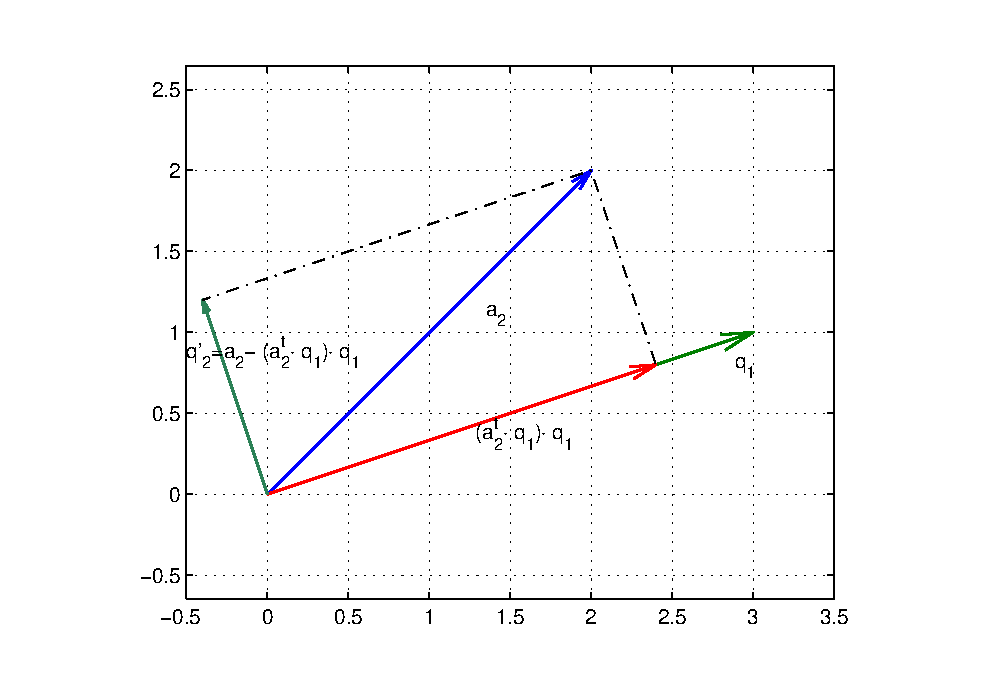
\includegraphics[width=12cm]{qr.eps}
\caption{Obtención de un vector ortogonal}
\label{fig:qr}
\end{figure}

Como $q_2$ tiene que ser un vector unitario para que la matriz $Q$ sea ortogonal, dividimos el vector obtenido, $q`_2$, por su módulo,

\begin{equation*}
q_2=\frac{V_2}{\lVert v_2 \rVert}=\frac{a_2-(q_1^T\cdot a_2)\cdot q_1}{\lVert a_2-(q_1^T\cdot a_2)\cdot q_1 \rVert}
\end{equation*}

Por último despejando $a_2$ podemos identificar los valores de $r_{12}$ y $r_{22}$, tal y como se describieron anteriormente,

\begin{align*}
a_2&= (q_1^T\cdot a_2)\cdot q_1+\lVert a_2-(q_1^T\cdot a_2)\cdot q_2 \rVert \cdot q_2\\
r_{12}&=q_1^T\cdot a_2\\
r_{22}&=\lVert a_2-(q_1^T\cdot a_2)\cdot q_2 \rVert 
 \end{align*}

Volviendo a la matriz $A$ de nuestro ejemplo la segunda columna de la matriz $Q$ y los valores de $r_{12}$ y $r_{22}$ quedarían,


\begin{align*}
q_2&=\frac{v_2}{\lVert v_2 \rVert}=\frac{a_2-(q_1^T\cdot a_2)\cdot q_1}{\lVert a_2-(q_1^T\cdot a_2)\cdot q_1 \rVert}=\left[\begin{pmatrix}
3\\
0\\
4
\end{pmatrix}-\frac{10}{3}\cdot \begin{pmatrix}
2/3\\
2/3\\
1/3
\end{pmatrix}\right]\cdot \frac{3}{5\sqrt{5}}=\frac{1}{5\sqrt{5}}\begin{pmatrix}
7/3\\
-20/3\\
26/3
\end{pmatrix}\\
r_{12}&=\frac{10}{3}\\
r_{22}&=\frac{5\sqrt{5}}{3}
\end{align*}
Se puede comprobar que los vectores $q_1$ y $q_2$ son ortogonales,
\begin{equation*}
q_1^T\cdot q_2= \begin{pmatrix}
2/3& 2/3& 273
\end{pmatrix}\cdot {5\sqrt{5}}\begin{pmatrix}
7/3\\
-20/3\\
26/3
\end{pmatrix}={5\sqrt{5}}\cdot \left(\frac{14}{3}-\frac{40}{3}+\frac{26}{3}\right)=0
\end{equation*}

Para obtener la tercera columna de la matriz $Q$, $q_3$ procederíamos de modo análogo: calcularíamos la proyección de la tercera columna de $A$, $a_3$ sobre los vectores formados por la los dos primeras columnas de $Q$, restamos de $a_3$ las dos proyecciones y normalizamos el vector resultante dividiéndolo por su módulo,

\begin{equation*}
q_3=\frac{v_3}{\lVert v_3 \rVert}=\frac{a_3-(q_1^T\cdot a_3)\cdot q_1-(q_2^T\cdot a_3)\cdot q_2}{\lVert a_3-(q_1^T\cdot a_3)\cdot q_1-(q_2^T\cdot a_3)\cdot q_2 \rVert}
\end{equation*} 

y de modo análogo al caso de la segunda columna,

\begin{align*}
r_{13}&=q_1^T\cdot a_3\\
r_{23}&=q_2^T\cdot a_3\\
r_{33}&=\lVert a_3-(q_1^T\cdot a_3)\cdot q_1-(q_2^T\cdot a_3)\cdot q_2 \rVert
\end{align*}

Es fácil observar como vamos obteniendo las sucesivas columnas de la matriz $Q$, iterativamente. Podemos generalizar los resultas anteriores para cualquier columna arbitraria de la matriz $Q$,

\begin{equation*}
q_i=\frac{a_i-\sum_{j=1}^i (q_j^T\cdot a_i)\cdot q_i}{\lVert a_i-\sum_{j=1}^i (q_j^T\cdot a_i)\cdot q_i \rVert}
\end{equation*}

y para los valores de $r_{1i}, r_{2i}, \cdots r{ii}$,
\begin{align*}
r_{ji}&=q_j^T\cdot a_i, \ j<i\\
r_{ii}&= \lVert a_i-\sum_{j=1}^i (q_j^T\cdot a_i)\cdot q_i \rVert
\end{align*}

El siguiente código de Matlab, calcula la factorización QR de una matriz, empleando el método descrito,

\begin{verbatim}
function [Q,R]=QRF1(A)
%%%%%%%%%%%%%%%%%%%%%%%%%%%%%%%%%%%%%%%%%%%%%%%%%%%%%%%%%%%%%%%%%%%%%%%%%%%
%Factorización QR obtenida directamente por ortogonalización de grand-schmidt
%Ojo, el algoritmo es inestable... Con lo que la bondad de las soluciones
%dependera de la matriz que se quiera factorizar.
%%%%%%%%%%%%%%%%%%%%%%%%%%%%%%%%%%%%%%%%%%%%%%%%%%%%%%%%%%%%%%%%%%%%%%%%%%%
%En primer lugar obtenemos las dimensiones de la matriz
[m,n]=size(A);

%fatorizamos columna a columna
for j=1:n
    %Construimos un vector auxiliar v, nos servira para ir obteniendo las
    %columnas de la matriz Q.
    for i=1:m %Solo llegamos hasta m factorización incompleta si m>n
        v(i)=A(i,j)
    end
    for i=1:j-1
        %obtenemos los elementos de la matriz R, correspondientes a la
        %columna j, solo podemos construir hasta una fila antes de la
        %diagonal i=j-1. cada fila es el producto escalar de la columna i
        %de la matriz Q for la columna j de la Matriz A.
        R(i,j)=0
        for k=1:m
        R(i,j)=R(i,j)+Q(k,i)*A(k,j)
        end
        
        %obtenemos las componentes del vector auxiliar que nos permitira
        %construir la columna j de la matriz Q
        for k=1:m
            v(k)=v(k)-R(i,j)*Q(k,i)
        end
    end
    %Obtenemos el valor del elemento de la diagonal R(j,j) de la matriz R

    R(j,j)=0
    for k=1:m
        R(j,j)=R(j,j)+v(k)^2
    end
    R(j,j)=sqrt(R(j,j))
    
    %Y por último, divimos los elementos del vector v por R(j,j), para
    %obtener la columna j de la matriz Q
    for k=1:m
        Q(k,j)=v(k)/R(j,j)
    end
end
\end{verbatim}
En general, el algoritmo que acabamos de describir para obtener la ortogonalización de Grand-Schmidt, es numéricamente inestable. La estabilidad puede mejorarse, si vamos modificando progresivamente la matriz $A$, a medida que calculamos las columnas de $Q$. 

Cada vez que obtenemos una nueva columna de $Q$, modificamos las columnas de $A$ de modo que sean ortogonales a la columna de $Q$ obtenida. Para ello, lo más sencillo es crear una matriz auxiliar $V$ que hacemos, inicialmente, igual a $A$, $V^{(0)}=A$

para obtener la primera columna de $Q$, procedemos igual que antes, normalizando la primera columna de $V^{(0)}$
\begin{align*}
q_1=\frac{v_1^{(0)}}{\lVert v_1^{(0)}\rVert}\\
r_{11}=\lVert v_1^{(0)}\rVert
\end{align*}

A continuación calculamos la proyección de todas las demás columnas de la matriz $V^{(0)}$ con respecto a $q_1$, esto es equivalente a calcular los restantes elementos de la primera fila de la matriz $R$: $r_{21}, r_{31}, \cdots r_{n1}$,
\begin{equation*}
r_{1j}=q_1^T\cdot v_j^{(0)}
\end{equation*}

Una vez calculadas las proyecciones, modificamos todas las columnas de $V^{(0)}$, excepto la primera restando a cada una su proyección con respecto a $q_1$.

\begin{equation*}
v_j^{(1)}=v_j^{(0)}-r_{1j}\cdot v_j^{(0)}, \ j=2,3,\cdot n
\end{equation*}

La nueva matriz $V^{(1)}$ cumple que todas sus columnas a partir de la segunda son ortogonales a $q_1$. Para obtener $q_2$ es suficiente dividir $v_2^{1}$ por su módulo,

\begin{align*}
q_2&=\frac{v_2^{(1)}}{\lVert v_2^{(1)} \rVert}\\
r_{22}&=\lVert v_2^{(1)} \rVert
\end{align*}

Podemos ahora calcular el resto de los elementos de la segunda fila de la matriz $R$ de modo análogo a como hemos calculado los de la primera,

\begin{equation*}
r_{2j}=q_2^T\cdot v_j^{(1)}
\end{equation*}

y, de nuevo actualizaríamos todos las columnas de $V^{1}$, a partir de la tercera, para que fueran ortogonales a $q_2$, 

\begin{equation*}
v_j^{(2)}=v_j^{(1)}-r_{2j}\cdot v_j^{(1)}, \ j=3,4,\cdot n
\end{equation*}

Las columnas de $V^{(2)}$ serían ahora ortogonales a $q_1$ y $q_2$. Si seguimos el mismo procedimiento n veces, calculando cada vez una nueva columna de $Q$ y una fila de $R$, obtenemos finalmente la factorización QR de la matriz inicial $A$. En general, para obtener la columna $q_i$ y los elementos de la fila $i$ de la matriz $R$ tendríamos,
 
\begin{align*}
q_i&=\frac{v_i^{(i-1)}}{\lVert v_i^{(i-1)} \rVert}\\
r_{ii}&=\lVert v_i^{(i-1)} \rVert
\end{align*}

\begin{equation*}
r_{ij}=q_i^T\cdot v_j^{(i-1)}
\end{equation*}

y la actualización correspondiente de la matriz $V$ sería,

\begin{equation*}
v_j^{(i)}=v_j^{(i)}-r_{ij}\cdot v_j^{(i)}, \ j=i+1,i+2,\cdot n
\end{equation*}

El resultado es el mismo que el que se obtiene por el primer método descrito. La ventaja es que numéricamente es más estable. 



El siguiente código de Matlab, calcula la factorización QR de una matriz de orden $n\times n$, empleando el método descrito,

\begin{verbatim}
function [Q,R]=QRF2(A)
%%%%%%%%%%%%%%%%%%%%%%%%%%%%%%%%%%%%%%%%%%%%%%%%%%%%%%%%%%%%%%%%%%%%%%%%%%%%
%Calculo de factorizacion QR de la matriz A, mediante la ortogonaliación de
%grand.schmidt modificada. Este algoritmo si que es estable...
%Obtenemos las dimensiones de A
%%%%%%%%%%%%%%%%%%%%%%%%%%%%%%%%%%%%%%%%%%%%%%%%%%%%%%%%%%%%%%%%%%%%%%%%%%%%
[m,n]=size(A);

%creamos una matriz auxiliar v sobre la que vamos a realizar la
%factorización. Se podría realizar directamente sobre A Machacando sus
%columnas según la factorización progresa... Sería lo correcto para ahorrar
%espacio de almacenamiento. Pero en fin, quizá así queda más claro aunque
%sea menos eficiente.
v=A;
%Como siempre, vamos factorizando por columnas de la matriz A


for i=1:m %la matriz Q tiene que ser mXm, aunque el numero de columnas de A sea n)
    %calculamos cada R(i,i) como el modulo del vector auxiliar v(1:m,i)
    R(i,i)=0;
    for k=1:m
        R(i,i)=R(i,i)+v(k,i)^2;
    end
    R(i,i)=sqrt(R(i,i));
    %calculamos el la columna i de la matriz Q, normalizando la columna i
    %de la matriz v
    for k=1:m
        Q(k,i)=v(k,i)/R(i,i);
    end
    %Modificamos todos los R(i,j) con ij>i, en cuanto tenemos la columna j
    %de la matriz Q, nos basta calcular el producto escalar con las
    %columnas de A (En nuestro caso de v porque están copiadas, de las
    %filas siguientes
    for j=i+1:n
        R(i,j)=0;
        for k=1:m
            R(i,j)=R(i,j)+Q(k,i)*v(k,j);
        end
        %i por último modificamos todas las columnas de la matriz v desde
        %i+1 hasta el final de la matriz. Aqui es donde cambia el algoritmo
        %ya que estamos modificando la matriz A, y las sucesivas matrices V
        %cada vez que obtenemos una nueva fila de valores de R
        for k=1:m
            v(k,j)=v(k,j)-R(i,j)*Q(k,i);
        end
    end
end
\end{verbatim}

Para terminar, indicar que Matlab tiene su propia función, \texttt{[Q,R]=qr(A)}, para calcular la factorización QR de una matriz. Para calcularla, emplea el método de ortogonalización de Householder. Este método es aún más robusto que la ortogonalización de Grand-Schmidt modificada. Pero no lo veremos en este curso. Damos a continuación un ejemplo de uso de la función \texttt{qr},
\begin{verbatim}
>> A=[2 3 1;2 0 2;1 4 3]

A =

     2     3     1
     2     0     2
     1     4     3

>> [q,r]=qr(A)

q =

   -0.6667    0.2087   -0.7155
   -0.6667   -0.5963    0.4472
   -0.3333    0.7752    0.5367


r =

   -3.0000   -3.3333   -3.0000
         0    3.7268    1.3416
         0         0    1.7889

>> q*r

ans =

    2.0000    3.0000    1.0000
    2.0000    0.0000    2.0000
    1.0000    4.0000    3.0000

\end{verbatim}
  
\subsection{Factorización SVD}\label{sec:SVD}
Dada una matriz cualquiera $A$ de orden $m\times n$ es posible factorizarla en el producto de tres matrices,
\begin{equation*}
A=U\cdot S \cdot V^T 
\end{equation*}

Donde $U$ es una matriz de orden $m\times m$ ortogonal, $V$ es una matriz de orden $n\times n$ ortogonal y $S$ es una matriz diagonal de orden $m\times n$. Además los elementos de $S$ son positivos o cero y están ordenados en orden no creciente,

\begin{equation*}
s=\begin{pmatrix}
\sigma_1& 0& \cdots & 0\\
0 & \sigma_2& \cdots & 0\\
\vdots & \vdots & \vdots & \vdots \\
0& 0& \cdots & \sigma_i\\ 
\end{pmatrix}; \ \sigma_1 \geq \sigma_2 \geq \cdots \geq \sigma_i; \ i=\min(m,n)
\end{equation*}

Los elementos de la diagonal de la matriz $S$, ($\sigma_1, \ \sigma_2, \  \cdots \ \sigma_i$), reciben el nombre de \emph{valores singulares} de la matriz $A$. De ahí el nombre que recibe esta factorización; SVD son las siglas en inglés de \emph{Singular Value Decomposition}.

No vamos a describir ningún algoritmo para obtener la factorización SVD de una matriz. En Matlab existe la función \texttt{[U,S,V]=svd(A)} que permite obtener directamente la factorización dSDV de una matriz $A$ de dimensión arbitraria. A continuación se incluyen unos ejemplos de uso para matrices no cuadradas,

\begin{verbatim}
>> A=[1 3 4;2 3 2;2 4 5;3 2 3]

A =

     1     3     4
     2     3     2
     2     4     5
     3     2     3

>> [U,S,V]=svd(A)

U =

   -0.4877    0.5175    0.1164   -0.6934
   -0.3860   -0.3612   -0.8375   -0.1387
   -0.6517    0.3024    0.0552    0.6934
   -0.4340   -0.7144    0.5311   -0.1387


S =

   10.2545         0         0
         0    1.9011         0
         0         0    1.1097
         0         0         0


V =

   -0.3769   -0.9170    0.1307
   -0.5945    0.1313   -0.7933
   -0.7103    0.3767    0.5946
\end{verbatim}

Como la matriz $A$ tiene más filas que columnas, la matriz $S$ resultante termina con na fila de ceros.

\begin{verbatim}
>> B=A'

B =

     1     2     2     3
     3     3     4     2
     4     2     5     3

>> [U,S,V]=svd(B)

U =

   -0.3769   -0.9170    0.1307
   -0.5945    0.1313   -0.7933
   -0.7103    0.3767    0.5946


S =

   10.2545         0         0         0
         0    1.9011         0         0
         0         0    1.1097         0


V =

   -0.4877    0.5175    0.1164   -0.6934
   -0.3860   -0.3612   -0.8375   -0.1387
   -0.6517    0.3024    0.0552    0.6934
   -0.4340   -0.7144    0.5311   -0.1387
   
\end{verbatim}

Como la matriz $B$, transpuesta de la matriz $A$ del ejemplo anterior, tiene más columnas que filas, la matriz $S$ termina con una columna de ceros.

A continuación enunciamos sin demostración algunas propiedades de la factorización SVD.

\begin{enumerate}
\item El rango de una matriz $A$ coincide con el número de sus valores singulares distintos de cero.
\item La norma-2 inducida de una matriz $A$ coincide con su valor singular mayor $\sigma_1$.
\item La norma de Frobenius de una matriz $A$ cumple:
\begin{equation*}
\lVert A \rVert_{F}=\sqrt{\sigma_1^2+\sigma_2^2+\cdots +\sigma_r^2}
\end{equation*}
\item Los valores singulares de una matriz $A$ distintos de cero son iguales a la raíz cuadrada positiva de los autovalores distintos de cero de las matrices $A\cdot A^T$ ó $A^T\cdot A$. (los autovalores distintos de cero de estas dos matrices son iguales),
\begin{equation*}
\sigma_i^2=\lambda_i(A\cdot A^T)=\lambda_i(A^T\cdot A)
\end{equation*}
\item El valor absoluto del determinante de una matriz cuadrada $A$,$n\times n$, coincide con el producto de sus valores singulares,
\begin{equation*}
\vert \det(A) \vert = \prod_{i=1}^n \sigma_i
\end{equation*}
\item El número de condición de una matriz cuadrada $A$ $n\cdot n$, que se define como el producto de la norma-2 inducida de $A$ por la norma-2 inducida de la inversa de $A$, puede expresarse como el cociente entre el el valor singular mayor de $A$ y su valor singular más pequeño,
\begin{equation*}
k(A)=\lVert A \rVert_2 \cdot \lVert A^{-1} \rVert_2 = \sigma_1 \cdot \frac{1}{\sigma_n}=\frac{\sigma_1}{\sigma_n}
\end{equation*}
El número de condición de una matriz, es una propiedad importante que permite estimar cómo de estables serán los cálculos realizados empleando dicha matriz, en particular aquellos que involucran directa o indirectamente el cálculo de su inversa.

\end{enumerate}
